% #############################################################################
% This is Chapter 6
% !TEX root = main.tex
% #############################################################################
% Change the Name of the Chapter i the following line
\fancychapter{Implications of Intelligent Agents}
\clearpage
% The following line allows to ref this chapter
\label{chap:chap006}

In this chapter, the implications of integrating {\it BreastScreening-AI} in a medical imaging workflow are detailed in terms of clinicians' performance and accuracy.
Recall, the {\it BreastScreening-AI} is a system-based on intelligent agents which are providing an automated diagnosis while integrating \ac{DL} methods on the \ac{UI} for medical imaging.
Here, three high-level goals are addressed:
i) how {\it receptive} are clinicians to the introduction of intelligent agents in medical imaging systems;
ii) how they {\it accept} and {\it interact} with these systems; and
iii) how an intelligent agent {\it affects} the \ac{UX} in the clinical context.
These high-level goals are addressed through a real-world case study of 45 clinicians from nine institutions.
Accuracy (measured in terms of \ac{FP} and \ac{FN} metrics) of intelligent agent results is compared and study the impact of the design techniques in the expectations and satisfaction of the clinicians.
Through an extensive experimental study, it was concluded that the proposed intelligent agent performed better than a traditional \ac{UI}, without a loss in diagnostic accuracy.

\section{Introduction}
\label{sec:sec006001}

Overstated expectations about \ac{UX} and usability decrease user acceptance and adoption of clinical systems, in particular when those expectations are not met~\cite{Inkpen:2019:HBG:3290607.3299002, Kocielnik:2019:YAI:3290605.3300641, Oh:2018:ILY:3173574.3174223}.
The recent hype of \ac{AI} techniques brings a new paradigm in the \ac{UX} context.
Modern assistant technologies, such as \ac{DL} methods opens new possibilities in the clinical domain~\cite{topol2019high}, including:
(i) genome interpretation~\cite{sundaram2018predicting};
(ii) medical coaching via a smart speaker ({\it e.g.}, Alexa)~\cite{bickmore2018patient};
(iii) assistive scan readings~\cite{madani2018deep};
(iv) cancer diagnosis and identification of mutations~\cite{coudray2018classification}; and
(v) mortality prediction~\cite{ahmad2018death}.
These methods exhibit good performance accuracy.
However, the underlying algorithms driving \ac{AI} functionalities are probabilistic and almost always operate at less than perfect accuracy.
Most clinicians do not expect their clinical systems to behave inconsistently and imperfectly~\cite{hoff2015trust, Kocielnik:2019:YAI:3290605.3300641}, which can lead to mistrust and potential abandonment of these technologies within real-world clinical setups~\cite{benrimoh2018aifred}.

Recently, \ac{DL} methods started outperforming traditional \ac{ML} algorithms in many application domains, where the access to large amount of data and training datasets was feasible.
The work described here is one such example. Specifically, a \ac{DL} methodology was introduced in a multi-modal breast imaging system.
To this end, {\it BreastScreening-AI} was developed as a multimodal medical imaging framework that allows radiologists and other clinicians to visualize and manipulate images, while also accessing a diagnostic recommendation from an \ac{AI} assistant.
The {\it BreastScreening} framework is used to test the usefulness of an intelligent medical agent that is integrated in an \ac{UI}.
For the work developed under this chapter, a large breast imaging database have been collected.
At that moment, the database contained 338 multi-modal image cases.
However, currently there are already more than 400 acquired cases.
Also, the database contains a dataset of manual delineation of the lesions ({\it i.e.}, ground-truth)
along with the classification of the lesion severity that is indexed on the \ac{BI-RADS}~\cite{ghosh2019artificial}.

As a means to provide an automatic classification of the exam using the \ac{BI-RADS}, intelligent agents are being integrated in the \ac{AI}-based diagnostic system ({\it BreastScreening-AI}),
Concealed by this system a \ac{DNN} was implemented following the DenseNet~\cite{chen2019learning} architecture.
To evaluate the diagnostic performance of the \ac{HAII} for the classification of breast cancer, {\it Precision} and  {\it Recall} metrics were used.
Using the {\it BreastScreening-AI} system, clinicians can {\it Accept} or {\it Reject} the assistant proposed \ac{BI-RADS} severity classification.

In this work, the results of applying {\it BreastScreening-AI} in a real-world scenario are presented, where radiologists and other clinicians can interact with the assistant ({\it i.e.}, DenseNet).
The assistant acts as a second reader, providing results in terms of improvements on the classification diagnosis ({\it i.e.}, Over-Diagnosis {\it vs} Under-Diagnosis) regarding \acp{FP} and \acp{FN}, as well as efficiency and efficacy in the workflow.
While considerable work as focused on improving the accuracy of \ac{AI} algorithms, comparatively less work focused on improving adoption and usability of interactive assistance techniques.
Making it a valuable topic to study, whereas the adjudication (Section~\ref{sec:sec003005}) of the final patient diagnostic is celebrated between the interaction of Humans and \ac{AI} (\ac{HAII}) algorithms.

Several high-level questions were asked according to this thesis, namely:
(i) how clinicians' respond to \ac{AI}-assistive medical imaging systems;
(ii) how they interact (and accept) with these systems; and
(iii) how \ac{AI}-assistive affects the \ac{UX} in the medical domain.
This thesis contributes broadly to the literature in \ac{HCI} and \ac{AI} by examining what clinicians need when using \ac{AI}-powered image diagnostic, the practices they adopt while using diagnostic tools, and how these diagnostic tools affect end-user attitudes towards the underlying \ac{AI} algorithms.

\section{Related Work}
\label{sec:sec006002}

From the retrieval of medical imaging data~\cite{faraji2019radiologic, seifabadi2019correlation}, medical imaging systems allow the end-user to diagnose several modalities.
In fact, by bringing several modalities together, it offers new possibilities for quantitative and qualitative imaging and diagnosis but also requires specialized data handling, post-processing and novel visualization methods~\cite{Igarashi:2016:IVS:2984511.2984537, Ocegueda-Hernandez:2016:CMN:2876456.2879485, Sousa:2017:VVR:3025453.3025566}.
Medical imaging tools, such as clinical assistants with intelligent agents, can help experts to make better decisions~\cite{Lopes:2017:UHC:3143820.3144118}, while identifying cancer prognostics among the available multi-modal data~\cite{lopes2018interaction}.
However, several challenges must be addressed for the introduction of such tools in the medical imaging domain.

A wide range of clinical assistants exist, providing clinicians with the knowledge to enhance the clinical workflow~\cite{Cai:2019:HTC:3290605.3300234, edge2019clinical}, from systems that supply potential information for medical decision-making ({\it e.g.}, \ac{CDSSe}) to those that make diagnostic decisions~\cite{hwang2019artificial}.
Although several studies have shown that an autonomous clinical assistant can reduce medical error and improve outcomes~\cite{Cai:2019:HTC:3290605.3300234, Cai:2019:EEE:3301275.3302289}, one traditional difficulty is to understand how user trust and acceptance is perceived during the diagnosis.

Experts may resist using an autonomous system if it does not capture the nuances of their mental models or provides relevant context~\cite{khairat2018reasons, kohli2018cad, yang2016investigating}.
On the other hand, clinicians are known to resist changes and new tools~\cite{10.1145/3132272.3134111, gagnon2014electronic}, an issue that has an impact in their workflow.
In this work, it focus on understanding different aspects and expectations of a medical imaging intelligent agent integrated into the radiology workflow.
In particular, the work demonstrates how an interactive \ac{AI} assistant can directly address the above mentioned issues during medical imaging diagnosis.
The following sections discuss recent advances on both \ac{HCI} and \ac{HAII} approaches.

\subsection{Explainability and Intelligibility}
\label{sec:sec006002001}

Most of the best performing autonomous clinical systems rely on \ac{ML} algorithms that learn specific tasks from training data.
The field recently gained enormous interest, mostly due to the practical successes of \ac{DL}~\cite{meacham2019towards}.
The rapid and widespread development of \ac{DL} methods supports a wide range of image analysis tasks, including classification, detection, and segmentation~\cite{lecun2015deep}.
These methods rely on large annotated data sets to learn and discriminate image features for each specific task, with performances matching and even surpassing human capabilities~\cite{esteva2017dermatologist}.

In medical applications, \ac{DL} has also been the major contributor to the success of these tools~\cite{esteva2019guide}, \textit{e.g.}, on the autonomous diagnosis of cancer~\cite{esteva2017dermatologist}, the segmentation of medical images~\cite{medley2019segmenting}, or breast cancer detection~\cite{MAICAS2019101562}.
Their outstanding performance in identifying meaningful patterns within the available data was recently used to help humans learn new biomarkers of specific diseases \cite{cole2017predicting,gonzalez2018deep,wang2019deep}, suggesting these models can see beyond what a trained radiologist sees in medical images.

Despite their success, autonomous systems are becoming increasingly more complex and incomprehensible to the users~\cite{holzinger2019causability}.
This gave rise to a critical challenge, particularly for medical applications, where results provided by an assistant does not explain the decision of the model~\cite{shah2019artificial}.
According to the literature, two approaches are currently proposed to address this challenge: \ac{XAI} and Intelligibility~\cite{gunning2017explainable, miller2018explanation}.
\ac{XAI} and Intelligibility, in the clinical context, must take into account that diverse data may contribute to a relevant result~\cite{Bharadhwaj:2019:ERS:3308557.3308699}.
One work~\cite{holzinger2018current} is addressing this need, underlining that clinicians must have the possibility to understand {\it how} and {\it why} a machine reached a given decision.
Moreover, transparent algorithms could appropriately enhance the trust of clinicians in future \acp{HAII}~\cite{Dominguez:2019:EEA:3301275.3302274, Weisz:2019:BTS:3301275.3302290}.

Transparency challenge gets much more complex when the output predictions are not obviously wrong~\cite{holzinger2018current}.
Considering the breast cancer domain, transparency seeks not just for an answer or output, but instead, it seeks for the diagnostic perdition that would require some kind of explanation (Section~\ref{sec:sec003006}) or structured adjudication (Section~\ref{sec:sec003006}) of the evidence used to support such prediction.
For instance, \acp{FP} can instill a lot of patient pressure and stress, but more importantly, \acp{FN} can make patient to die.
In order to support explicit computation that produces a model explanation of the predicted output, the challenge is about {\it how} to construct more explicit models and {\it what} are clinicians learning from it.

\subsection{Human-In-The-Loop}
\label{sec:sec006002002}

Although the research concerning interaction with intelligent systems is recent~\cite{burr2018analysis, johnson2016face}, still this topic has seen new advances {\it e.g.}, chat-bots and other agents~\cite{chattopadhyay2017evaluating, miller2019intrinsically, mou2017media}.
Recent advances in medical technologies that promote the generation of data, have continued to drive interaction research in the clinical domain~\cite{azuaje2019artificial, chin2018clinical}.
Moreover, the new interest of the medical community to support \ac{AI} research projects and the available public datasets, are encouraging researchers to work on both fields~\cite{lau2018dataset, price2018big}.

\ac{HAII} incorporates human feedback in the training process to create better \ac{ML} models.
The topic is also known as \ac{iML}~\cite{fails2003interactive} or \ac{HITL}~\cite{holzinger2016interactive}.
In this work, it refers to the topic as \ac{HAII}, that somehow is addressed in~\cite{10.1145/3290605.3300233} providing a set of design guidelines.
In the work developed by Kocielnik et al.~\cite{Kocielnik:2019:YAI:3290605.3300641}, the authors are also addressing their study with the impact of several methods of expectation setting, and others studied the design for specific \ac{HAII} scenarios~\cite{aha2017ai}.
While much of the mentioned prior work has employed handcrafted features~\cite{10.1145/3290605.3300233, Kocielnik:2019:YAI:3290605.3300641}, the thesis leverage rich image data features automatically learned from \ac{DL} algorithms.

By focusing on the clinical domain, it is argued that \ac{HAII} research could improve clinical recommendation systems and clinical decision-making~\cite{holzinger2019interactive}.
Giving clinicians access to \ac{AI} systems, requires mechanisms to understand the machine decision process.
While this thesis can assume that expert clinicians are always able to explain their decisions, it is interesting to know that sometimes they are not able to provide a clear explanation.
One explanation is the vast amount of data sources and their diversity~\cite{Bharadhwaj:2019:ERS:3308557.3308699, lau2018dataset, price2018big}.
Consequently, \ac{HAII} calls for confidence and trust, bringing usability into a new and vital focus of \ac{AI} systems.

\section{Research Questions}
\label{sec:sec006003}

Since the research questions, herein formulated, are strongly related with the performance metrics, the work starts by defining them within the medical context.
The accuracy level of a clinical system is defined as the total number of correct predictions over all possible predictions~\cite{seref2019performance}.
This definition requires  the use of the following error metrics:
(1) \ac{FP}; and
(2) \ac{FN}.
Typically, both \acp{FP} and \acp{FN} are quantified as {\bf Precision} {\it vs} {\bf Recall}, respectively.
Generally, clinical systems are optimized for high precision and, therefore, avoid \acp{FP} ({\it i.e.}, in breast context, avoid recommending a \ac{BI-RADS} higher than the real one).

Previous works outside of the clinical scope~\cite{Kocielnik:2019:YAI:3290605.3300641, Dove:2017:UDI:3025453.3025739}, denote that the impact of \ac{FP} {\it vs.} \ac{FN} on \ac{UX} is generally unexplored.
However, thus is of high relevance when considering \ac{AI} systems for the clinical domain~\cite{boughey2016identification, dialani2015role} as it will be experimentally shown.
This thesis also want to measure that the proposed assistant as a function of the above metrics.
Measuring predictions are typically quantified as precision in contrast with recall.
Therefore, this work explore the following \underline{R}esearch \underline{Q}uestions and associated each to the set of \underline{H}ypothesis accoirding to the guidelines described in~\cite{10.1145/3290605.3300233, Kocielnik:2019:YAI:3290605.3300641}.

\noindent
Specifically, it was considered the following research questions and related hypothesis:

%%%%%%%%%%%%%%%%%%%%%%%%%%%%%%%%%%%%%%%%%%%%%%%%%%%
\begin{itemize}
\item {\bf RQ6.1.} What is the impact and acceptance of \ac{AI} on the medical workflow with respect to the perceived \ac{UX} of clinicians?

An AI system where the perceived \ac{UX} of clinicians is focused on Precision/Recall will result in:

\begin{itemize}
\item {\bf H6.1.1.} higher accuracy.
\item {\bf H6.1.2.} higher acceptance.
\end{itemize}
\item {\bf RQ6.2.} How does the Precision/Recall of an \ac{AI} system affects receptiveness from clinicians and their expectations for the perception of what the system can do?

Clinicians' receptiveness and expectations of the system capabilities are affected by:

\begin{itemize}
\item {\bf H6.2.1.} rates of \acp{FP}.
\item {\bf H6.2.2.} rates of \acp{FN}.
\item {\bf H6.2.3.} time performance for \acp{FP}.
\item {\bf H6.2.4.} time performance for \acp{FN}.
\end{itemize}
\item {\bf RQ6.3.} What are clinicians' inter-variability and intra-variability during patient classification?
\begin{itemize}
\item {\bf H6.3.1.} The inter-variability is improved by the introduction of \ac{AI}.
\item {\bf H6.3.2.} The intra-variability is improved by the introduction of \ac{AI}.
\end{itemize}
\end{itemize}
%%%%%%%%%%%%%%%%%%%%%%%%%%%%%%%%%%%%%%%%%%%%%%%%%%%

\hfill

The work in~\cite{10.1145/3290605.3300233}, describes a set of \underline{18 guidelines} (Table~\ref{tab:tab004}) for \ac{HAII} being highly useful to support the remaining research questions.
Also, in~\cite{Kocielnik:2019:YAI:3290605.3300641} it is provided  an exploratory study of an assistant to study the impact of several methods of user expectations.
In both studies, the authors show that different focus on avoiding types of errors lead to a quite different subjective perceptions of accuracy and acceptance.
Prior work of the authors~\cite{Kocielnik:2019:YAI:3290605.3300641} shows three significant contributions to clinician's expectations:
(1) information from external sources;
(2) reasoning and understanding; and
(3) first hand experience.
From here, this thesis aims to explore design techniques for achieving these mechanisms pairwise with the work done in~\cite{10.1145/3290605.3300233}.
Also, the thesis provides an opportunity to reflect on practices in a specific case of \ac{HAII} early in its clinical context.

%%%%%%%%%%%%%%%%%%%%%%%%%%%%%%%%%%%%%%%%%%%%%%%%%%%
\begin{table}[htbp]
\centering
\resizebox{\columnwidth}{!}{%
\begin{tabular}{|l|l|l|l|}
\hline
\multicolumn{4}{|c|}{AI Design Guidelines}                                                                    \\ \hline
G1 & Make clear what the system can do.                    & G10 & Scope services when in doubt.              \\ \hline
G2 & Make clear how well the system can do what it can do. & G11 & Make clear why the system did what it did. \\ \hline
G3 & Time services based on context.                       & G12 & Remember recent interactions.              \\ \hline
G4 & Show contextually relevant information.               & G13 & Learn from user behavior.                  \\ \hline
G5 & Match relevant social norms.                          & G14 & Update and adapt cautiously.               \\ \hline
G6 & Mitigate social biases.                               & G15 & Encourage granular feedback.               \\ \hline
G7 & Support efficient invocation.                         & G16 & Convey the consequences of user actions.   \\ \hline
G8 & Support efficient dismissal.                          & G17 & Provide global controls.                   \\ \hline
G9 & Support efficient correction.                         & G18 & Notify users about changes.                \\ \hline
\end{tabular}
}
\caption{The 18 human-AI interaction design guidelines~\cite{10.1145/3290605.3300233}. These guidelines were validated by the authors through multiple rounds of evaluation.}
\label{tab:tab004}
\end{table}
%%%%%%%%%%%%%%%%%%%%%%%%%%%%%%%%%%%%%%%%%%%%%%%%%%%

For {\bf RQ6.1}, this thesis want to explore the impact of proposed assistant avoiding errors concerning clinicians' accuracy and acceptance.
Under this work, it was explored how the system, with a focus on {\it High Precision}, can result in both higher accuracy and acceptance.
Last, the thesis mapped~\cite{10.1145/3290605.3300233} the {\bf H6.1.1} with {\bf G1}, {\bf G2} and {\bf G3} guidelines.
On the other hand, the work mapped the {\bf H6.1.2} hypothesis with {\bf G5}, {\bf G6} and {\bf G7} guidelines.

The {\bf RQ6.2} question evaluates the effectiveness of the expectation adjustment techniques in increasing clinicians' satisfaction with the system after using the assistant for completing actual diagnostic.
This thesis will foresee that more accurate expectations of an \ac{AI} system capabilities should result in clinicians being better prepared for \ac{AI} system imperfections and, therefore, result in higher satisfaction and performance.
For these question hypotheses, enumerated as {\bf H6.2.1}, {\bf H6.2.2}, {\bf H6.2.3} and {\bf H6.2.4}, the hypothesis were mapped it with {\bf G8}, {\bf G9} and {\bf G10} guidelines.

Finally, measurements of {\bf RQ6.3} will answer what the clinicians' inter-variability and intra-variability during patient classification with the introduction of \ac{AI}.
To achieve better results, the work aims to mitigate clinicians' biases and understand user behaviour.
The proposed assistant must provide granular feedback and global controls, notifying clinicians about changes.
Moreover, it need to show contextually relevant information making clear what the system can do.
For that, the system adapted the assistant cautiously by conveying the consequences of user actions.
As follows, the applied guidelines are presented for this {\bf RQ6.3}.
First of all, the {\bf H6.3.1} was mapped with {\bf G6}, {\bf G12}, {\bf G15}, {\bf G17} and {\bf G18} guidelines.
Second and final, the {\bf H6.3.2} was mapped with {\bf G4}, {\bf G11}, {\bf G13}, {\bf G14} and {\bf G16} guidelines.
Mapping these guidelines will orient this work to prototype an assistant that we expect to reduce inter-variability and intra-variability of clinicians.
Next, details of the assistant will be provided.

\section{Medical Assistant Framework}
\label{sec:sec006004}

The proposed {\it BreastScreening-AI} framework incorporates an assisted tool ({\it i.e.}, an intelligent agent for severity classification) offering radiologists a second opinion reader during the breast cancer diagnosis that is accomplished  using  a DenseNet model~\cite{chen2019learning}.
To validate the proposed DenseNet results, the framework allows the radiologist to {\it accept} or {\it reject} the proposed \ac{BI-RADS} classification.
Therefore, the radiologist can freely control the final diagnosis result.
The {\it BreastScreening-AI} platform operates as a website that can be accessed via a web browser.
In fact, a web browser-based solution is covering the early concerns regarding remote and distributed (Section~\ref{sec:sec004002004}) requirements of this thesis.

\subsection{Design Choices}
\label{sec:sec006004001}

Due to the multi-view and multi-modal nature of the data, the proposed assistant uses large amounts of images.
The most common used modalities are as follows:
(i) \ac{US} (both \ac{CC} and \ac{MLO} views);
(ii) \ac{US}; and
(iii) \ac{MRI} volumes.
The above modalities results from a selection provided by the radiologists team.
Notice that in (i) a large number of \ac{MG} views are available, {\it e.g.}, MG-ML, MG-LM, MG-LMO, late MG-ML, among others.
Concerning (iii), the acquisition allows to obtain a large set of \ac{MRI} data ({\it e.g.}, T1, T2, \ac{DCE})~\cite{seifabadi2019correlation}.

Initial design choices resulted in a consensus that allowed the selection of \ac{CC} and \ac{MLO} views, in the case of MG, 
and \ac{DCE} for the case or \ac{MRI}.
From the above, it is vital to have the \textit{5.1.~Viewports} management feature (Figure~\ref{fig:fig040}), providing the users with the opportunity to arrange the viewport depending on the available modalities and views.
Furthermore, the thesis choose to implement the \textit{5.2.~Toolbars} with a quick and configurable \textit{5.1.~Viewports} management button, to support this use case.

%%%%%%%%%%%%%%%%%%%%%%%%%%%%%%%%%%%%%%%%%%%%%%%%%%%
\begin{figure}[htbp]
\centering
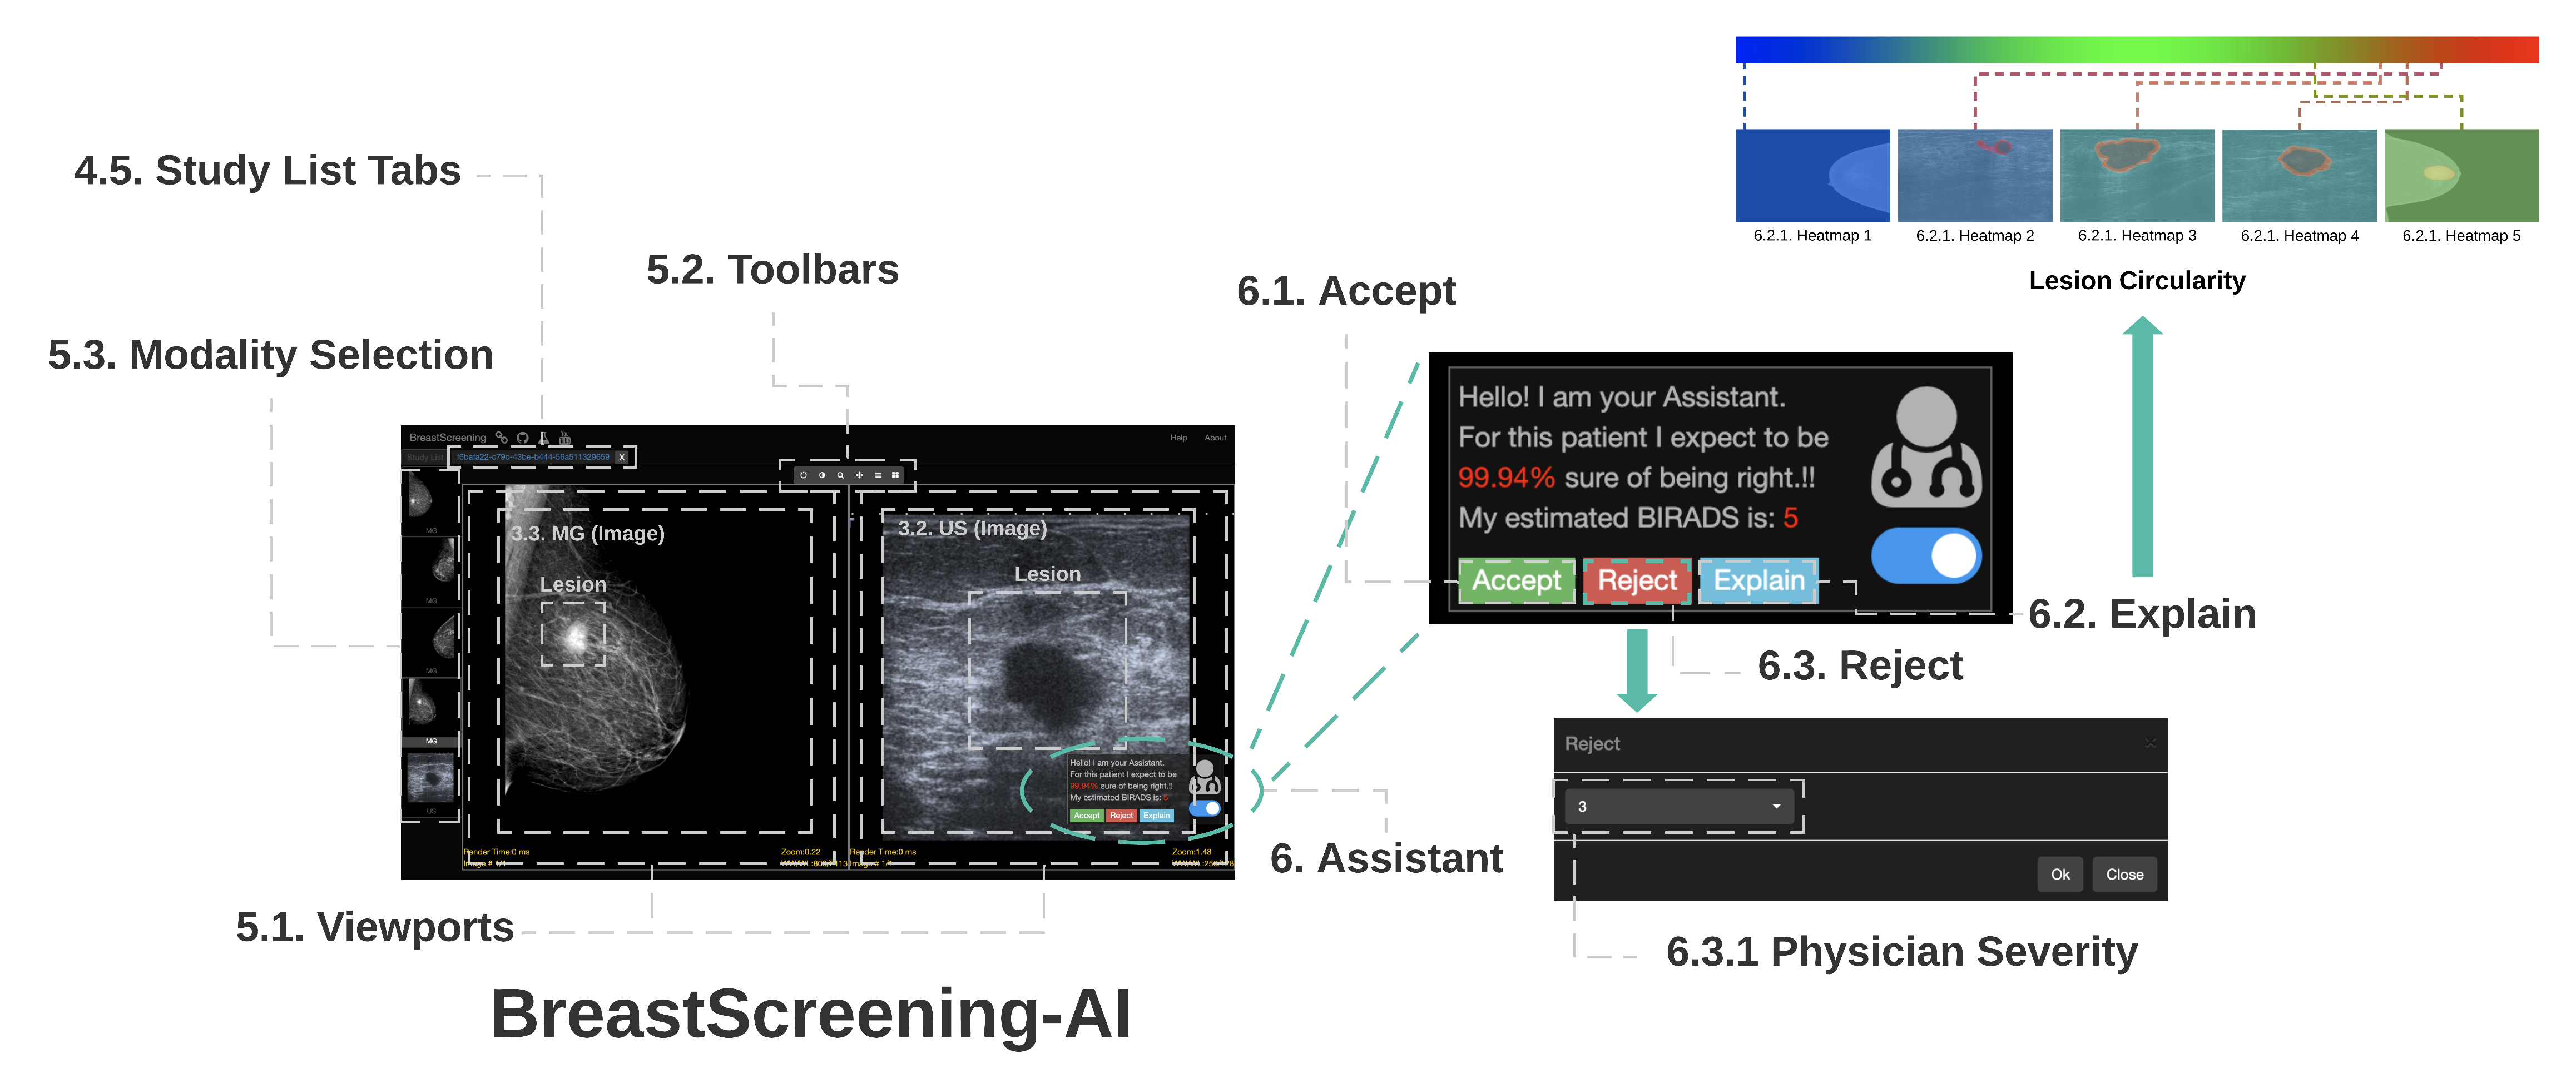
\includegraphics[width=\textwidth]{images/fig040}
\caption{The proposed {\it BreastScreening-AI} provides several functionalities. Specifically, it is possible to validate the DenseNet output classification along with radiologists. The system is framed in the following subcategories: 4.5. Study List Tabs; 5.1. Viewports; 5.2. Toolbars; 5.3. Modality Selection; 6. Assistant; 6.1. Accept; 6.2. Explain; 6.3. Reject; and 6.3.1. Physician Severity. On 6.2. Explain, the assistant will pop-up several heatmaps. The proposed model has two main stages: (i)  first it computes the BI-RADS, based on the output classification of the DenseNet; and (ii) it computes the size and circularity of the lesion based on the heatmaps.}
\label{fig:fig040}
\end{figure}
%%%%%%%%%%%%%%%%%%%%%%%%%%%%%%%%%%%%%%%%%%%%%%%%%%%

For breast cancer, the user evaluation validated design choices (Section~\ref{sec:sec006006}) and revealed clinician strategies for using the intelligent agent as a medical assistant.
The learned design lessons should, in principle, generalize to other healthcare assisted systems.
Design lessons are further discussed (Section~\ref{sec:sec006007}) to understand how patterns of user interactions with {\it BreastScreening-AI} helped to highlight some of more common clinician groups ({\it i.e.}, Interns, Juniors, Middles and Seniors) and behaviours.
In the end, these patterns are also discussed and mapped to other healthcare assisted systems.

\subsection{User Interface}
\label{sec:sec006004002}

Based on the user needs, {\it BreastScreening-AI} was designed and implemented.
Specifically, the tool is including a set of refinement mechanisms to guide radiologists during the diagnostic process.
The designed \ac{UI} of {\it BreastScreening-AI} consists of one main component, comprising the medical imaging views (Figure~\ref{fig:fig040}).

The {\it 4.5. Study List Tabs} (Figure~\ref{fig:fig040}) gives radiologists the opportunity to switch between the patient who is being diagnosed and a full list of patients.
Using the {\it 5.2.~Toolbars} on the {\it 5.1.~Viewports}, the clinician can locate the lesions and classify its severity (via \ac{BI-RADS}), choosing the {\it 6.1.~Accept} or {\it 6.3.~Reject} options for the given severity of the {\it 6.~Assistant}.

When the several modalities are correctly used (regarding the {\it 5.3.~Modality~Selection} on a multimodality view), the clinician can find more accurately the right severity classification.
For the {\it 6.3.~Reject} option, the clinician will have to insert the proposed \ac{BI-RADS} on a drag-and-drop menu ({\it 6.3.1.~Physician Severity}) of severity options.
Finally, the clinician may look for the {\it 6.2.~Explain} feature (Figure~\ref{fig:fig040}) showing the model explainability regarding the {\it Lesion Circularity} values.
In the following sections, the sections will be explaining how to measure the {\it Lesion Circularity}.

\subsection{Implementation}
\label{sec:sec006004003}

{\it BreastScreening-AI} framework was implemented using CornerstoneJS\footnotemark[36]~\cite{urban2017lesiontracker} with a NodeJS framework\footnotemark[37]~\cite{farrell2016nodejs, drnasin2017javascript} and ExpressJS\footnotemark[38]~\cite{gustin2017empowerment} for managing the server part.
To sustain the system and user evaluation, image sets are selected from Hospital Fernando Fonseca (Section~\ref{sec:sec005005001}) and uploaded them into an Orthanc server~\cite{Jodogne2018}.
Patient data was collected from this institution.
Then, a user evaluation method was followed and applied~\cite{https://doi.org/10.13140/rg.2.2.16566.14403/1} to the remaining nine (Section~\ref{sec:sec005005001}) clinical institutions.
Three imaging modalities (\ac{MG}, \ac{US} and \ac{MRI}) were provided for each patient.
The images were pre-processed and anonymized on the Orthanc server and then consumed by the system.
This system is efficiently designed as a set of modules (Figure~\ref{fig:fig041}) that can be reused in other imaging applications.

%%%%%%%%%%%%%%%%%%%%%%%%%%%%%%%%%%%%%%%%%%%%%%%%%%%
\footnotetext[36]{\href{https://cornerstonejs.org/}{cornerstonejs.org} - a JavaScript library to display interactive medical images of the assistant including but not limited to DICOM. It was used to display the medical images on the browser. Accessed on 8th of December, 2020.}
%%%%%%%%%%%%%%%%%%%%%%%%%%%%%%%%%%%%%%%%%%%%%%%%%%%

%%%%%%%%%%%%%%%%%%%%%%%%%%%%%%%%%%%%%%%%%%%%%%%%%%%
\footnotetext[37]{\href{https://nodejs.org}{nodejs.org} - a JavaScript based framework for back-end implementation. NodeJS is defined as a JavaScript code execution environment. Accessed on 8th of December, 2020.}
%%%%%%%%%%%%%%%%%%%%%%%%%%%%%%%%%%%%%%%%%%%%%%%%%%%

%%%%%%%%%%%%%%%%%%%%%%%%%%%%%%%%%%%%%%%%%%%%%%%%%%%
\footnotetext[38]{\href{https://expressjs.com}{expressjs.com} - minimal and flexible NodeJS web application framework that provides a robust set of features. It deals with requests, responses and subsequent middleware functions. Accessed on 8th of December, 2020.}
%%%%%%%%%%%%%%%%%%%%%%%%%%%%%%%%%%%%%%%%%%%%%%%%%%%

The CornerstoneJS family of libraries provide essential functions, such as
i) image rendering;
ii) \ac{DICOM} retrieval;
iii) tool support ({\it i.e.}, developed functionalities); and
iv) interpretation.
Additionally, the {\it BreastScreening} core (Section~\ref{sec:sec004004001001}) was developed in JavaScript with jQuery\footnotemark[39]~\cite{depeursinge2011mobile} for \ac{HTML} document manipulation, event handling of the \ac{UI} interactions, such as mouse events, and with look \& feel improvements.

%%%%%%%%%%%%%%%%%%%%%%%%%%%%%%%%%%%%%%%%%%%%%%%%%%%
\footnotetext[39]{\href{https://jquery.com}{jquery.com} - a fast, small, and feature-rich {\it JS} library for the GUI. {\it JQuery} is generic, as it can be configured to render many different types of views.}
%%%%%%%%%%%%%%%%%%%%%%%%%%%%%%%%%%%%%%%%%%%%%%%%%%%

Additionally, a {\it dicomParser}~\cite{zhang2015dicom} was used for parsing \ac{DICOM} files.
The \ac{DICOM} files can be loaded by drag-and-drop into the browser window on the Orthanc  (Figure~\ref{fig:fig041}) view.
Loaded images can be further displayed on both views, but with different visualization configurations.
After loading stage, images are automatically arranged according to the scan IDs from the \ac{DICOM} files.

%%%%%%%%%%%%%%%%%%%%%%%%%%%%%%%%%%%%%%%%%%%%%%%%%%%
\begin{figure}[htbp]
\centering
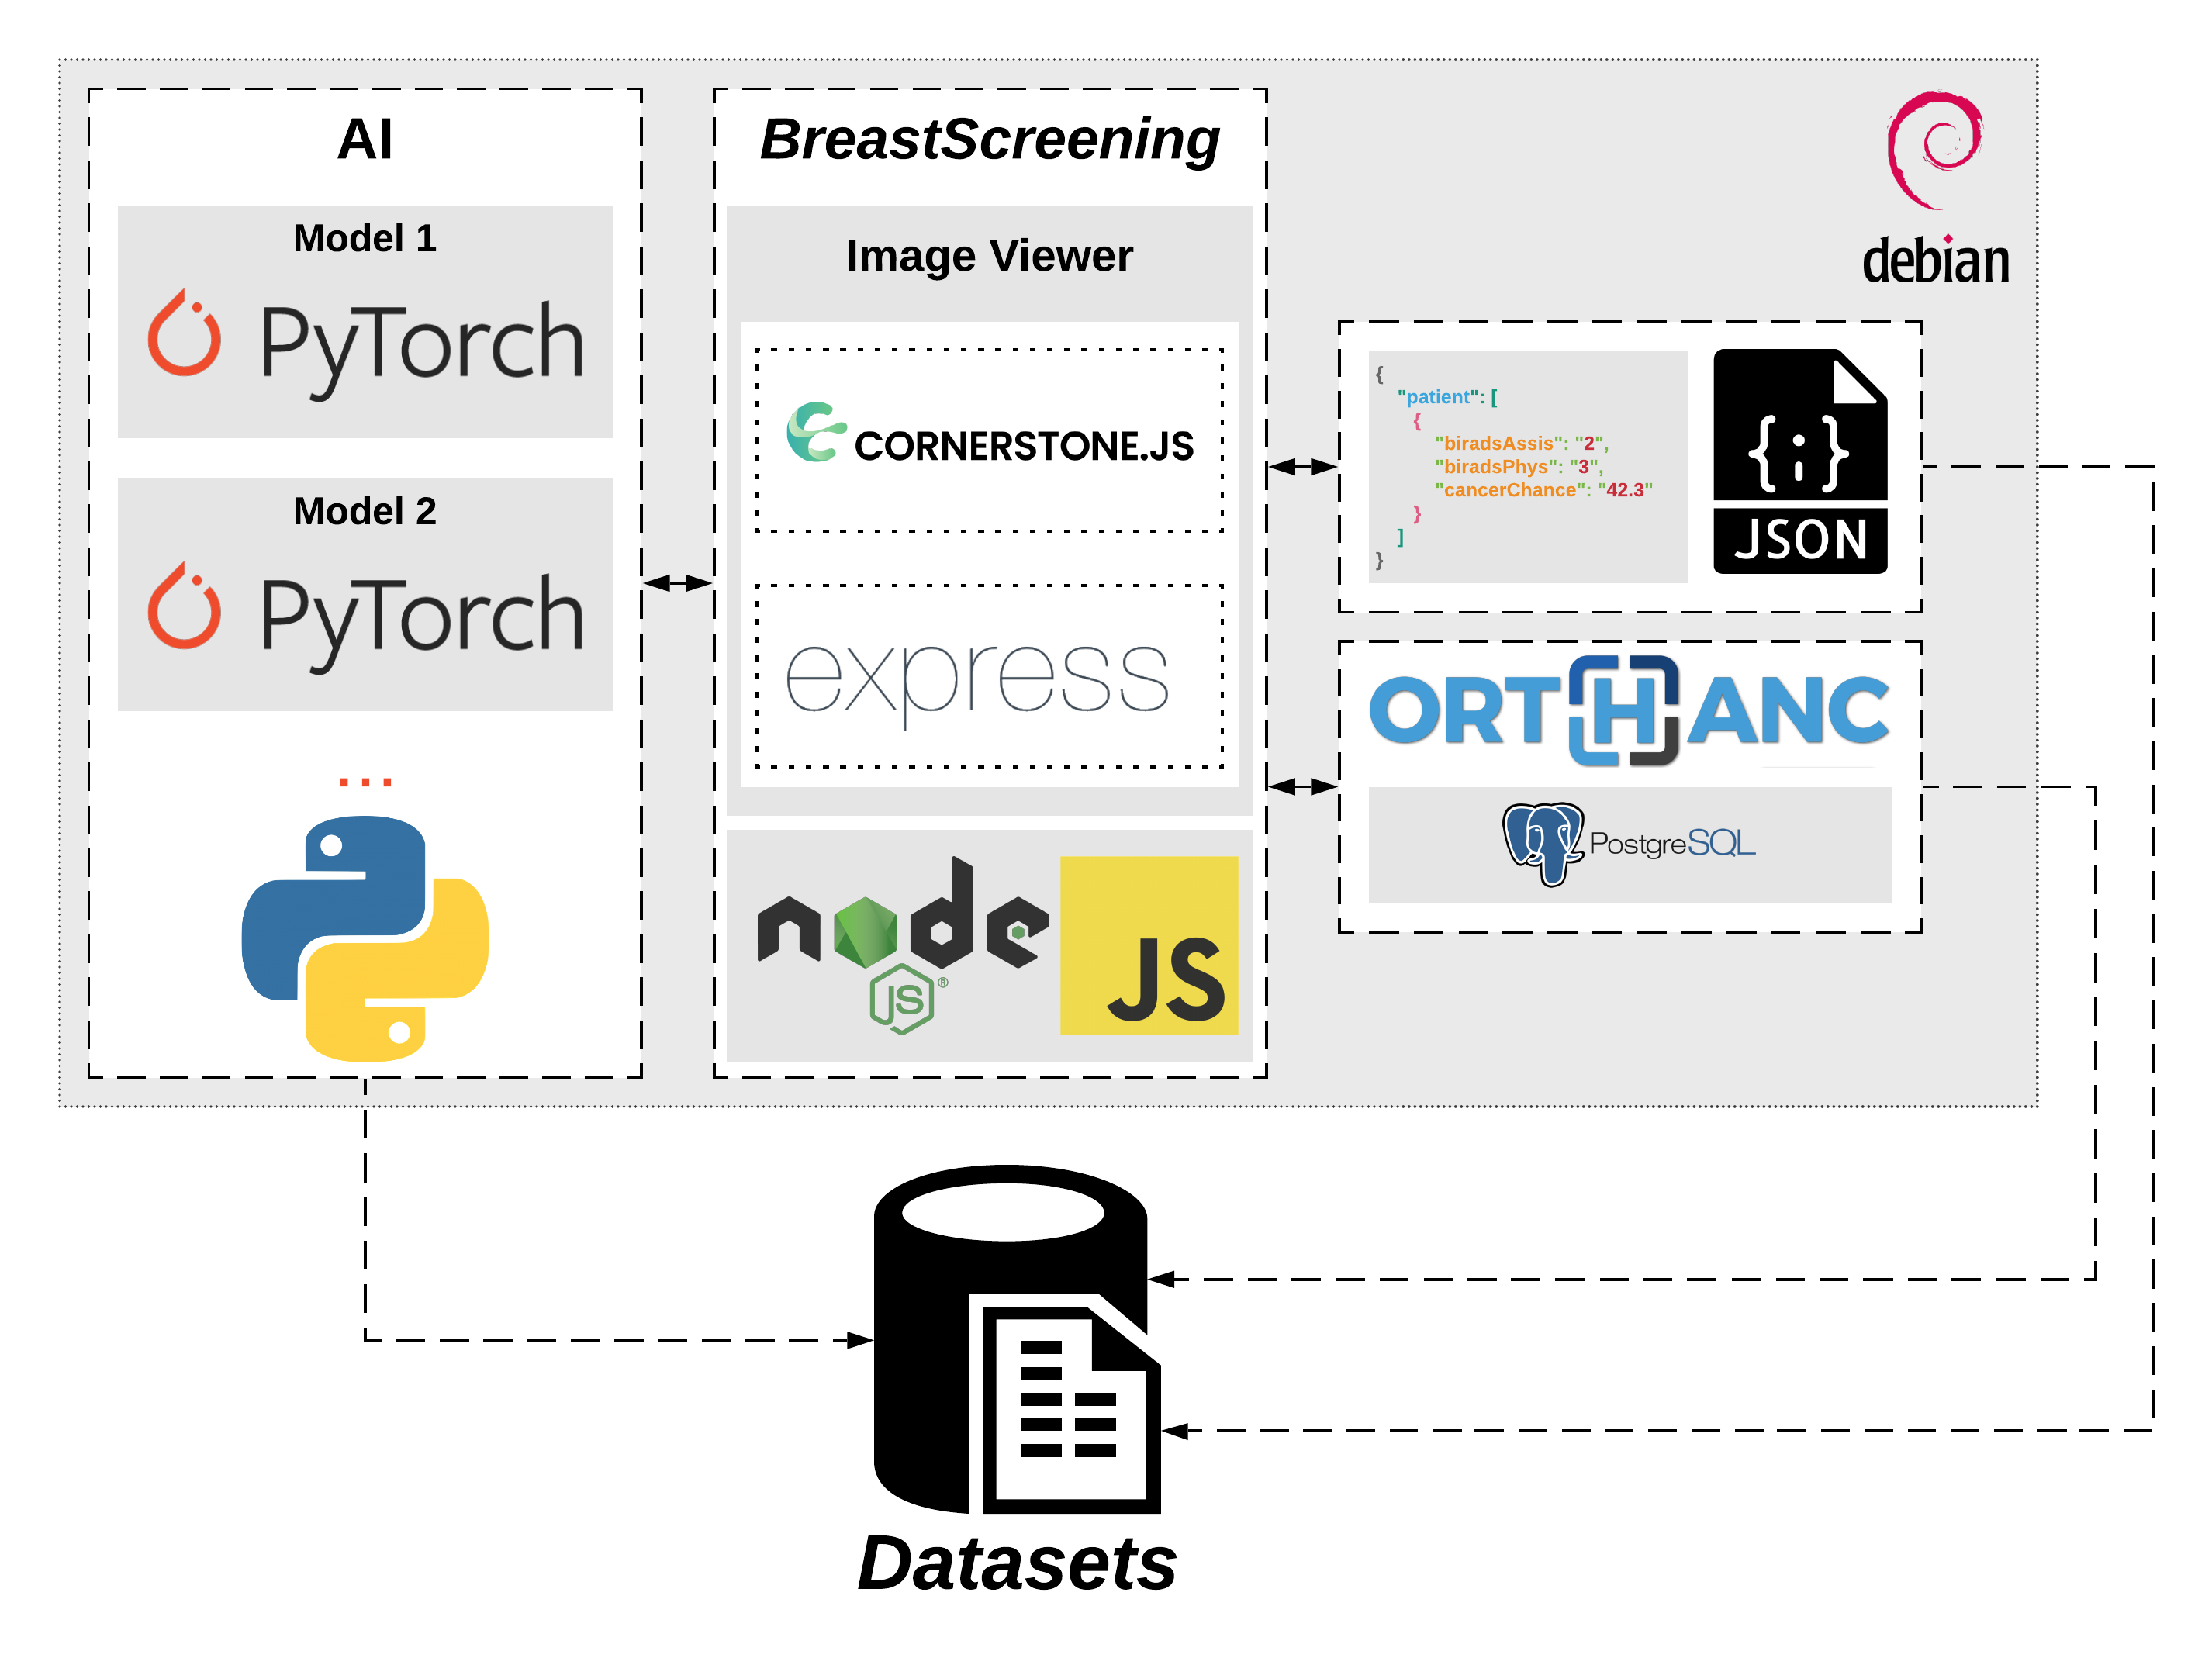
\includegraphics[width=0.95\linewidth]{images/fig041}
\caption{{\it BreastScreening-AI} Architecture: the main components of the system are AI Application, Image Viewer, Datasets and DICOM Storage. The Image Viewer of {\it BreastScreening} framework will provide essential interaction tools for radiologists. A study list is fetched from the Orthanc server, and through CornerstoneJS the radiologist can manipulate the image, interacting with the assistant at the same time.}
\label{fig:fig041}
\end{figure}
%%%%%%%%%%%%%%%%%%%%%%%%%%%%%%%%%%%%%%%%%%%%%%%%%%%

Finally, for this assistant, the DenseNet was developed using \href{https://pytorch.org/}{PyTorch}~\cite{NEURIPS2019_bdbca288}.
More specifically, \href{https://pytorch.org/}{PyTorch} is a \ac{DL} library that is widely used by the \ac{ML} community due to its imperative and ``Pythonic'' programming style.
The library performs immediate execution of dynamic tensor computations with automatic differentiation and \ac{GPU} acceleration, and does so while maintaining performance comparable to the fastest current libraries for \ac{DL} methods.
The availability and normalization of general-purpose massively parallel hardware, such as \acp{GPU}, provided the computing power required to this thesis.
Thus, \href{https://pytorch.org/}{PyTorch} was used under this work  (Figure~\ref{fig:fig041}) to facilitate the implementation of \ac{DL} methods and easily integrate the methods into intelligent agents.

\subsection{Acquired Medical Imaging Datasets}
\label{sec:sec006004004}

In order to control the medical imaging information, radiologists interact with in a sub-sequence study.
The {\it BreastScreening-AI} was fixed to operate on a limited subset of 289 classified patients from the collected dataset at Hospital Fernando Fonseca.
In fact, the acquired dataset of medical images contains more than 200 000 \ac{DICOM} files from a total of 338 patients.
For this work, each of the 289 patients was classified by the head of radiology of Medical Imaging Department at Hospital Fernando Fonseca.
Then, the head of radiology expert provided both \ac{BI-RADS} values of the pre-biopsy and pathological results of each patient.

From the pre-biopsy classification, the acquired and curated dataset was divided into three distinct patient types:
{\bf P1} with low severity, {\it i.e.}, BIRADS $\leq$ 1;
{\bf P2} with medium severity, {\it i.e.}, 1 $<$ BIRADS $\leq$ 3; and
{\bf P3} with high severity, {\it i.e.}, BIRADS $>$ 3;
on all possible modalities (\ac{MG}, \ac{US} and \ac{MRI}).
Each radiologist will open each patient ({\it e.g.}, {\bf P1}, {\bf P2} or {\bf P3}), that is chosen randomly, and will examine the set of images.
The dataset resulted from work done by eight of the 45 clinicians.
All of the eight clinicians are resident radiologists of Hospital Fernando Fonseca working directly with the head of radiology of this institution.

\subsection{Model Description}

A fundamental component in the designed \ac{UI} is the integration of a \ac{DNN} ({\it i.e.}, DenseNet).
A DenseNet is capable to automatically provide the classification for the lesion severity of the exam.
For this study, the DenseNet~\cite{Huang_2017_CVPR} architecture used in {\it BreastScreening-AI} was DenseNet-161 (Figure~\ref{fig:fig012}).
The DenseNet was initially pre-trained on ImageNet~\cite{10.1145/3351095.3375709}, a large dataset of 1.2 million images from 1,000 classes.
This is an important step, to regularize the network whenever small sets are available for training.
The network parameters were fine-tuned using the acquired and curated medical dataset.
This is accomplished by removing the last layer and replace it by a new fully-connected layer for five classes, corresponding to the \ac{BI-RADS} (from 1 to 5) values.

For fairness purposes the curated dataset was splitted into two disjoint sets: training and testing sets.
The training is used to fine-tune the weights of the architecture to the medical dataset acquired and curated under this thesis.
The test is an hold-out set used exclusively for testing.
Notice that, in the experimental evaluation only the test set is used, where the radiologists are asked to perform the patient ({\it i.e.}, {\bf P1}, {\bf P2} or {\bf P3}) diagnosis.

%%%%%%%%%%%%%%%%%%%%%%%%%%%%%%%%%%%%%%%%%%%%%%%%%%%
\begin{figure}[htbp]
\centering
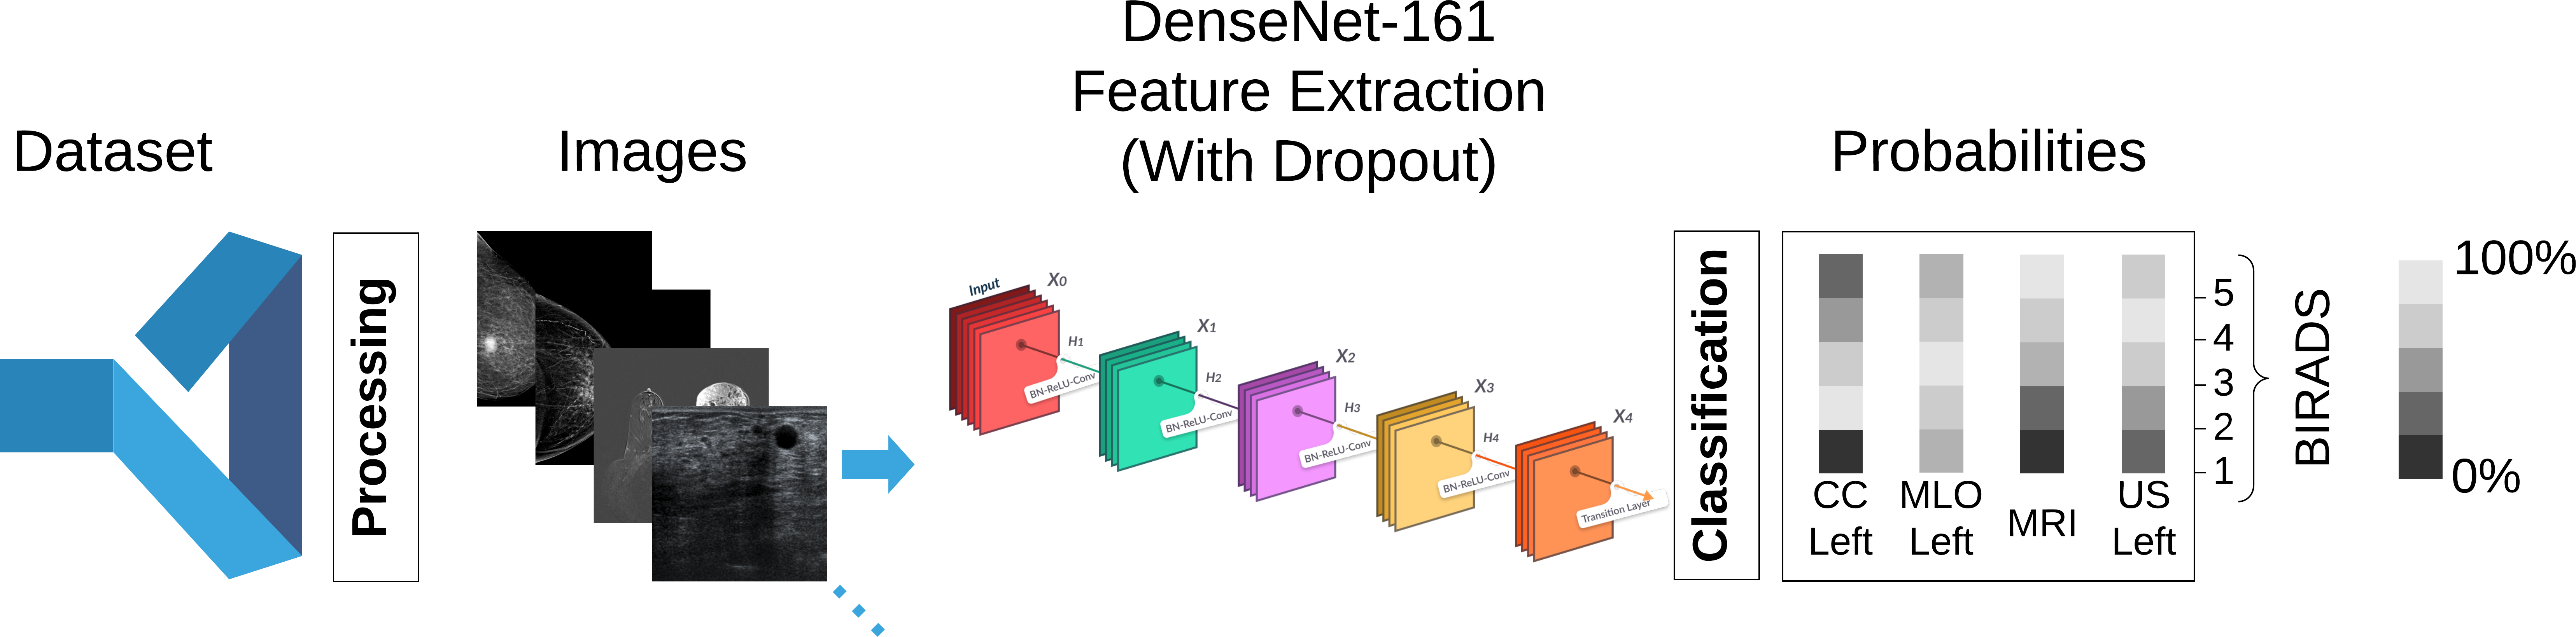
\includegraphics[width=\textwidth]{images/fig042}
\caption{DenseNet extracts features from images using dense blocks to efficiently compute the probability of each class. Classification probabilities are calculated and, in the end, the intelligent agent display the highest probability ({\it i.e.}, from 0\% to 100\%) of all images from that patient. Moreover, the resulted Classification/Probabilities square can also be displayed to provide some kind of XAI to clinicians.}
\label{fig:fig042}
\end{figure}
%%%%%%%%%%%%%%%%%%%%%%%%%%%%%%%%%%%%%%%%%%%%%%%%%%%

All modalities were evaluated by the same model, and required a pre-processing step, which included resizing the images to $224\times 224$ pixels (with bilinear interpolation), as well as normalization which removed the mean and standard deviation.
Similarly to what was done for ImageNet.
Training was performed using the Adam optimizer~\cite{kingma2014adam}, with the default parameters (learning rate of $10^{-3}$ and weight decay of $10^{-4}$).

Online data augmentation was also used to prevent over-fitting, namely by using random cropping (with a 10 pixel zero-padding on each side) and random horizontal flipping.
To train the model, the cross-entropy loss was used, in which the model predictions (after softmax) were compared to the classifications provided by the team of radiologists.
At test time, the unseen images went through the same pre-processing step mentioned above.
Both the model predictions (\textit{i.e.}, the probability assigned to each class, which expresses the model confidence in that classification) and the classification (most probable class) were stored.
With this setup, the model achieved an accuracy of 94.81\% on the test set.

\section{Methods}
\label{sec:sec006005}

{\it BreastScreening-AI} was evaluated while simulating real-world conditions with 45 clinicians in nine different clinical institutions.
The goal of this work was to quantitatively and qualitatively assess the proposed design principles that the {\it BreastScreening-AI} system embodies (rather than on particular widgets of the \ac{UI}) and to understand how these principles would fare in practice.
This thesis was particularly interested in understanding how {\it BreastScreening-AI} would accomplish improvements of diagnosis, surpassing the challenges and providing evidence of the opportunities emerging from \ac{HAII}.
Ultimately, the thesis is focused on radiologists' accuracy while using the proposed {\it BreastScreening-AI} functionalities and how to improve \ac{AI} reliability during medical decision-making.

\subsection{Participants}
\label{sec:sec006005001}

As the above study (Chapter~\ref{chap:chap005}), participants were asked to practice with three predefined patients ({\it i.e.}, {\bf P1}, {\bf P2} and {\bf P3}).
Then, participants were asked to diagnose each patient.
Recall that these patients belong to the test set, that have never been seen by the DenseNet.
The assistant is expected to minimize the time required and accuracy ({\it e.g.}, better \ac{FP} or \ac{FN} values).

The study of this Chapter~\ref{chap:chap006} involved also the same 45 clinicians, recruited on a volunteer basis from a broad range of clinical scenarios (Section~\ref{sec:sec005005001}), including nine different health institutions (two public hospitals, two cancer institutes and two private clinics).
Again, from the demographic questionnaires:
24.44\% of the clinicians have between 31 and 40 years of practical experience (Seniors);
31.11\% have between 11 and 30 years of experience (Middles);
17.78\% have between 6 and 10 years of experience (Juniors); and
26.67\% have limited experience (Interns).
Interviews were conducted in a semi-structured fashion taking about 30 minutes per clinician.
Overall, the team spent 57 days on the clinical institutions for the observation process and six months for the classification.

\subsection{Apparatus}
\label{sec:sec006005002}

To track user interactions across the evaluated system, the \hyperlink{https://www.hotjar.com/}{Hotjar}~\cite{liikkanen2017data} tool was used.
This tool is an analytic package allowing this study to follow users remotely.
It also provides two critical pieces of functionality, among others, that can aid in remote user testing.
First of all, the frequency areas allow us to see where users are clicking, tapping and scrolling on the system.
Second, it records a video playback of the entire user session.
The tool shows evidence of being useful for the studies conducted herein.
To record the task activities and the interview, the \hyperlink{https://support.apple.com/downloads/quicktime}{QuickTime} application was used for user's screen recording.

Finally, to understand radiologists' reading behaviour an eye-tracking device was used while they were interacting with the intelligent agent.
The selected device was the \hyperlink{https://gaming.tobii.com/product/tobii-eye-tracker-4c/}{Tobii Eye Tracker 4C}, since Tobii is the largest commercial eye tracking manufacturer, and is one of the most common trackers among usability practitioners~\cite{sidenko2018eye}.
Also, the \hyperlink{https://www.tobiipro.com/product-listing/tobii-pro-sdk/}{Tobii Pro SDK}~\cite{chatelain2018evaluation} was used, providing the thesis results with gaze information of the eye tracking device.

\subsection{Analysis}
\label{sec:sec006005003}

For this study, both quantitative and qualitative analysis were conducted.
The quantitative analysis focused on measuring the radiologists' performance ({\it e.g.}, number of \acp{FP} and \acp{FN}) during diagnosis of three groups of patients ({\it i.e.}, low, medium and high severity) for each doctor.
The above measurements are part of the quantitative analysis with a comparison between {\it Clinician-Only} and {\it Clinician-AI} setups.
Both setups will be further detailed.

To do a detailed comparison, the study will answer the research questions and hypothesis mentioned in Section~\ref{sec:sec006003}, providing evidence for the impact, expectations and acceptance of \ac{AI} assistance on the \ac{RRR} workflow.
For the qualitative analysis, opinion-based feedback was extracted from the recorded audio during the interaction with the prototype.
The content analysis that led to a set of key-phrases, was expressed as the number of clinicians who shared similar opinions.

\subsection{Procedure}
\label{sec:sec006005004}

In this study, within-subjects design was used to compare the performance of both {\it Clinician-Only} and {\it Clinician-AI} setups.
Succinctly, clinicians first assess the three patients ({\it i.e.}, spread by Low, Medium and High severities) on the {\it Clinician-Only} setup and then, with other three patients, on the {\it Clinician-AI} setup.
Tasks were derived from test scenarios developed from use cases and/or with the assistance of a subject-matter expert.
The tasks are identical for all participants of a given user role in the study.

Each participant interacts with the assistant, {\it accepting} or {\it rejecting} the system suggestion, that is, the output classification of the \ac{DNN}.
The test set will comprise a number of 289 patients, where each patient in the set must have at least one of the three available modalities.
Each participant will open the respective set of three patients ({\it e.g.}, {\bf P1}, {\bf P2} or {\bf P3}), chosen randomly, and will examine the set of images.
During the examination, the participant will interact with the available functionalities (Figure~\ref{fig:fig040}) of the system.

\subsection{Quantitative Measures}
\label{sec:sec006005005}

System accuracy was measured through three questions adapted from the Model of Trust~\cite{schoorman2016perspective} that is mentioned here as \ac{DOTS}: (1) {\bf Understanding}: "{\it I understand what the system is thinking}"; (2) {\bf Capability}: "{\it The system seems capable}"; and (3) {\bf Benevolence}: "{\it The system seems benevolent}".
The three questions were answered on a 20-point scale from "{\it 0\% - Totally Disagree}" to "{\it 100\% - Totally Agree}" with 5\% increments.
Several {\it post-task} questions were done, such as usability and workload questions (between others).

The {\it post-task} questions, aim to evaluate satisfaction, were adapted from~\cite{Kocielnik:2019:YAI:3290605.3300641}: {\it How well the assistant worked?}, that is important to the Model of Trust~\cite{basheer2015certainty, khalid2016prediction}.
Result metrics of recall and precision of the system were also measured.
Then, it was applied a standard analysis to determine the effect of the attributes on the clinician's interpretation and expectations.
To have a fair measure of the system performance, the \ac{GT} of the real \ac{BI-RADS} values (provided by the head of the radiology department) was calculated and used as a comparison metric.
From the \ac{GT}, the number of \acfp{TP}, \acfp{TN}, \acfp{FP} and \acfp{FN} were computed.

In order to take further conclusions of the acquired data, the following performance measures are summarized as: \underline{R}ecall (R = \ac{TP} / (\ac{TP} + \ac{FN})), \underline{P}recision (P = \ac{TP} / (\ac{TP} + \ac{FP})).
For instance, if a clinician provides a \ac{BI-RADS} of 3 but the real \ac{BI-RADS} is a 5 we consider it as an \ac{FN} result.
On the other hand, if the real \ac{BI-RADS} is a 2 but the clinician provides a \ac{BI-RADS} of 4 we consider it as an \ac{FP} result.
Another factor to take into account is that the \ac{BI-RADS} is a scale, {\it i.e.}, it has an order.
This means that, if the model says the \ac{BI-RADS} is 3 ({\it i.e.}, {\it Medium} severity), when the real \ac{BI-RADS} is 5 ({\it i.e.}, {\it High} severity), it should be less serious than the model saying it is a \ac{BI-RADS} of 1 ({\it i.e.}, {\it Low} severity).

\section{Results}
\label{sec:sec006006}

In this section, the section experimentally shows the usefulness of integrating the Human-\ac{AI}, namely its gains when compared to the single radiologist performance.
The experimental evaluation will be conducted to map the \acp{RQ} formulated in Section~\ref{sec:sec006003}.
The study will comprise on the following setups.
The collaboration (within-subject) was distributed into three scenarios: (i) {\it Clinician-Only}; (ii) {\it Clinician-AI}; and (iii) {\it AI-Only}.
For each scenario, three patient classes are considered.
Concretely, {\it Low}, {\it Medium} and {\it High} severities.
Each class concerns the lesion severity in the \ac{BI-RADS} score, as ${\rm BIRADS} = 1$, ${\rm BIRADS} \in\{2, 3\}$ and, ${\rm BIRADS}\in\{4, 5\}$, respectively.

\subsection{RQ6.1 - Clinical Impact}
\label{sec:sec006006001}

Concerning the first research question (RQ6.1), Figure~\ref{fig:fig043} and Figure~\ref{fig:fig044} show the metric statistics using the confusion matrix (with 45 clinicians).
More precisely, the performance accuracy can be observed with the proposed \ac{AI} integration (Figure~\ref{fig:fig043}) is superior in comparison with the performance without integration (Figure~\ref{fig:fig044}).
In this confusion matrix, the diagonal shape of the matrix is denoted as being more evident with the introduction of the \ac{AI} (Figure~\ref{fig:fig043}).
Moreover, the diagnostic accuracy is also higher (Table~\ref{tab:tab005}) when the assistant is integrated in the \ac{UI}.
The mean and standard deviation\footnotemark[40] of (M = 0.656, SD = 0.34) and 
(M = 0.622, SD = 0.27) were obtained for the {\it Precision} and {\it Recall}, respectively.
From the above results, the hypothesis {\bf H6.1.1} is therefore supported.

%%%%%%%%%%%%%%%%%%%%%%%%%%%%%%%%%%%%%%%%%%%%%%%%%%%
\footnotetext[40]{{\it N}: the number of users (Clinicians); $F\textsubscript{var}$: the F-test used for comparing the factors of the total deviation per each variable ({\it var}) categorized by clinical experience; $M\textsubscript{var}$: Mean value of the variable ({\it var}); $SD\textsubscript{var}$: the Standard Deviation (SD) per each variable ({\it var}) denoted in this description of the results.}
%%%%%%%%%%%%%%%%%%%%%%%%%%%%%%%%%%%%%%%%%%%%%%%%%%%

%%%%%%%%%%%%%%%%%%%%%%%%%%%%%%%%%%%%%%%%%%%%%%%%%%%
\begin{table}[htbp]
\centering
\begin{tabular}{|c|c|c|c|c|c|c|}
\hline
\multirow{2}{*}{BIRADS} & \multicolumn{2}{c|}{Precision} & \multicolumn{2}{c|}{Recall} & \multicolumn{2}{c|}{F1-score}   \\ \cline{2-7} 
                        & Clini.-On.      & Clini.-AI    & Clini.-On.     & Clini.-AI    & Clini.-On.     & Clini.-AI    \\ \hline
1                       & 0.01            & 0.69         & 0.76           & 0.91         & 0.02           & 0.78         \\ \hline
2                       & 0.13            & 0.86         & 0.91           & 0.91         & 0.23           & 0.88         \\ \hline
3                       & 0.20            & 0.50         & 0.50           & 0.20         & 0.29           & 0.29         \\ \hline
4                       & 0.20            & 0.99         & 0.61           & 0.68         & 0.30           & 0.81         \\ \hline
5                       & 0.99            & 0.99         & 0.57           & 0.86         & 0.72           & 0.92         \\ \hline
\end{tabular}
\caption{Reported performance of Clinician-Only (Clini.-On.) and Clinician-AI (Clini.-AI) collaborations. The {\it Precision} is the fraction of relevant instances among the classified instances. On the other hand, the {\it Recall} (sensitivity) is the fraction of relevant instances classified over the total amount of relevant instances. The {\it F1-score} is the harmonic mean of precision and recall, giving a balanced measure of precision and recall performance.}
\label{tab:tab005}
\end{table}
%%%%%%%%%%%%%%%%%%%%%%%%%%%%%%%%%%%%%%%%%%%%%%%%%%%

From the \ac{DOTS}~\cite{https://doi.org/10.13140/RG.2.2.23078.37448/1} questionnaire\footnotemark[41], 98\% of the 45 clinicians answered that they do understand what the system is thinking.
Also, 93\% of the clinicians trust on the system capability, answering {\bf H6.1.2} regarding the acceptance of the system.
Using \ac{DOTS}~\cite{10.1145/2898375.2898385}, it was possible to answer the two null-hypotheses of {\it an \ac{AI} system focused on Precision/Recall will result in}: (1) {\bf H6.1.1} higher accuracy; and (2) {\bf H6.1.2} higher acceptance.

%%%%%%%%%%%%%%%%%%%%%%%%%%%%%%%%%%%%%%%%%%%%%%%%%%%
\footnotetext[41]{The DOTS is a 3-item Likert scale questionnaire. In this study, the three questions are scored between 0 and 20.}
%%%%%%%%%%%%%%%%%%%%%%%%%%%%%%%%%%%%%%%%%%%%%%%%%%%

%%%%%%%%%%%%%%%%%%%%%%%%%%%%%%%%%%%%%%%%%%%%%%%%%%%
\begin{figure}[htbp]
\centering
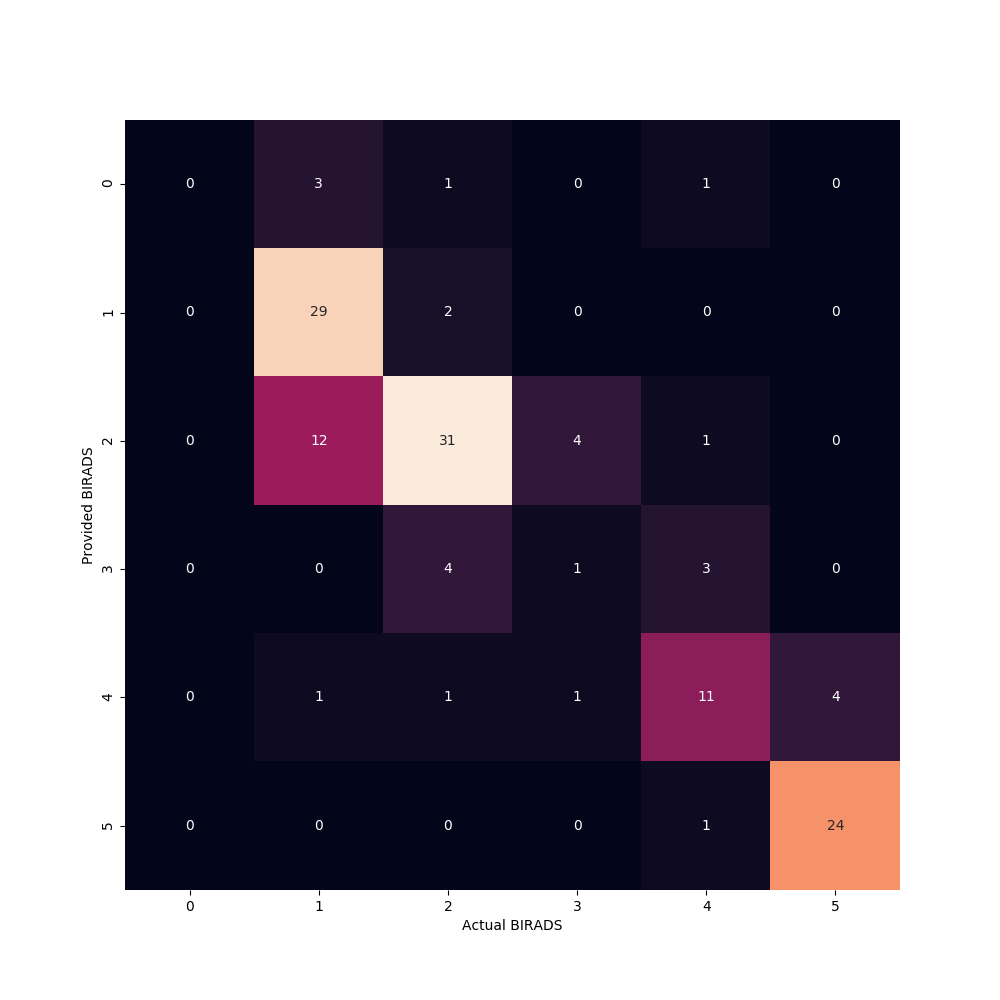
\includegraphics[width=\textwidth]{images/fig043}
\caption{Confusion Matrix with information of the collaboration ({\it Provided}) between physicians and the proposed AI ({\it Clinician-AI}) technique. For this case, a DenseNet results were used among the BI-RADS outputs to support the physician decision. The classification accuracy was 71\% for the number of True-Positives. On the other hand, the number of False-Negatives was 15\% and the number of False-Positives was 14\%, only. The {\it Provided} value was most accurate in classifying low (BIRADS $<$ 2) and high (BIRADS $\ge$ 4) severity cases. The columns represent the {\it Actual} (biopsy confirmed) category of the objects and the rows represent the {\it Provided} (collaboration between physician and AI) value.}
\label{fig:fig043}
\end{figure}
%%%%%%%%%%%%%%%%%%%%%%%%%%%%%%%%%%%%%%%%%%%%%%%%%%%

%%%%%%%%%%%%%%%%%%%%%%%%%%%%%%%%%%%%%%%%%%%%%%%%%%%
\begin{figure}[htbp]
\centering
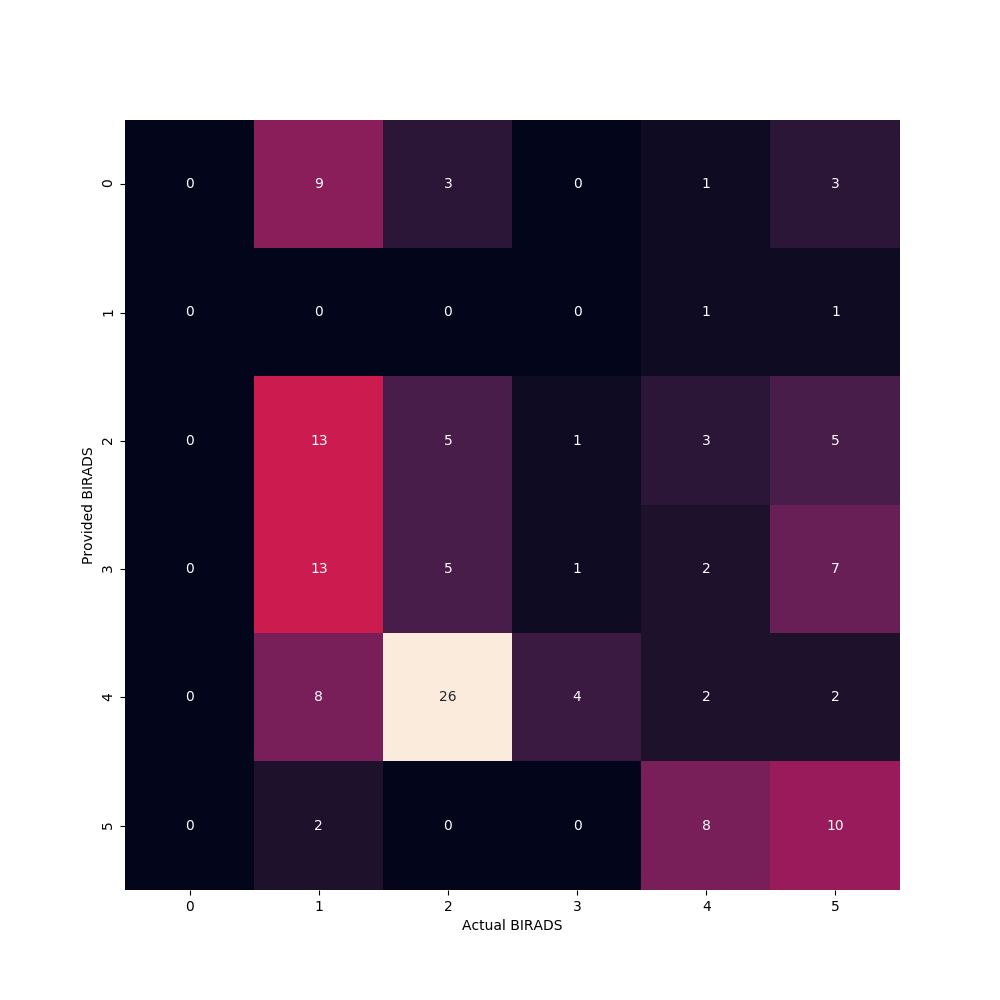
\includegraphics[width=\textwidth]{images/fig044}
\caption{Confusion Matrix without the AI ({\it Clinician-Only}) technique. For this case, the DenseNet results were not used. Each physician directly provided the BI-RADS to the system with no support of AI techniques. The classification accuracy was just 13\% for the number of True-Positives. On the other hand, the number of False-Negatives was 59\% and the number of False-Positives was 28\%. The {\it Provided} value was most accurate in classifying high (BIRADS $\ge$ 4) severity cases. The columns represent the {\it Actual} (biopsy confirmed) category of the objects and the rows represent the {\it Provided} (only physician) value.}
\label{fig:fig044}
\end{figure}
%%%%%%%%%%%%%%%%%%%%%%%%%%%%%%%%%%%%%%%%%%%%%%%%%%%

\subsection{RQ6.2 - User Expectations}
\label{sec:sec006006002}

Concerning the explanation (\ac{XAI}) for clinicians, a visual information strategy was adopted that relies on the use of {\it heatmaps} (Figure~\ref{fig:fig032}).
Herein, the work takes into consideration the following two functionalities for the colored-visualization:
(1) the lesion circularity or distribution; and
(2) the associated \ac{BI-RADS} value.
It is known that the mass morphology is a relevant feature for the lesion classification~\cite{maicas2018training}.
The more irregular the lesion is, the more severe its classification will be.
Thus hot colors are associated to more irregular morphology, improving the user's expectation regarding the final result of the \ac{AI}.
Concerning the \ac{BI-RADS}, we also assign hot colors for increasing values of the \ac{BI-RADS}. 
This can be easily accomplished by the clinician, by simply press the {\it 6.2. Explain} button.

From the \ac{DOTS} questionnaire, the following scores for {\bf Understanding} were obtained.
Concretely, (M = 19.7, SD = 2.92) and (M = 10, SD = 7) when clinicians {\it press} or {\it do not press} the  {\it Explain} button, respectively.
Furthermore, the values of trust in the assistant were also much higher (M = 18.81, SD = 2.96) in comparison to the values of clinicians who did not press the {\it 6.2. Explain} button (M = 12.43, SD = 3.21).
Similarly no significant imbalance was present in prior frequency for the use of {\it BreastScreening-AI}.
That said, the {\bf RQ6.2} was considered as covered.

Explanation intervention is significantly increasing clinicians’ perceived level, both in terms of understanding and trust capability.
This suggests that an assistant design helps to improve user perception.
Another important requirement for the clinician's acceptance is to provide the control of the system.
This can be accomplished by assigning to the {\it control} with {\it Accept} or {\it Reject} functionalities as a way to provide (or inhibit) a second opinion, resulted by the assistant.
From \ac{DOTS}, the answers to this questionnaire obtained 76\% of the clinicians that agreed to {\it Accept} with a positive benevolence statistics (M = 14.67, SD = 5.24).
In this work, by providing clinicians' with control of the final result, it revealed a significant (p $<$ 0.05) positive impact, with a higher feeling of control for clinicians that agree with the benevolence of the assistance than for those that did not agree.
Now analysing the 14\% of clinicians who did {\it Reject}, it should be highlighted that from this set, 52\% of the clinicians failed (M = 3.72, SD = 4.68) in the classification, contributing for the higher \acp{FP} or \acp{FN} rates.

Finally, it was found that the integration of the assistant helps clinicians to improve the final rates, {\it i.e.}, \acp{FP} and \acp{FN} ({\bf H6.2.1} and {\bf H6.2.2}), and time performance ({\bf H6.2.3} and {\bf H6.2.4}).
This is related with the number of correctly identified cases during the classification (Figure~\ref{fig:fig043} and Figure~\ref{fig:fig044}) that is always higher than the ones obtained without the assistant.
Specifically, the mean values of (M = 19.2, SD = 12.81) and (M = 3.6, SD = 4.03) were obtained, with and without the assistance, respectively.
The values are taken from the diagonal of the confusion matrices.
Furthermore, in terms of time performance (Section~\ref{sec:sec005006001005}), it can be denoted that with the {\it Clinician-AI} (M = 76.67 seconds, SD = 85.96 seconds) setup clinicians took less time in comparison to the {\it Clinician-Only} (M = 113.33 seconds, SD = 66.64 seconds) setup.

With the above results, both {\bf H6.2.1} and {\bf H6.2.2} hypotheses were considered as supported.
In terms of time performance, clinicians took 31\% less diagnostic time with the assistant (M = 308 seconds, SD = 57.03 seconds) in comparison with no assistance (M = 377 seconds, SD = 44.56 seconds).
Reflecting an improvement of 69 seconds per image, which does not seems much, but for patients with more than 10 images (something really common), it will save more than 11 minutes per patient.
Therefore, the current result can answer the two {\bf H6.2.3} and {\bf H6.2.4} null-hypotheses since improvements of time performance were achieved in both \acp{FP} and \acp{FN}.
Achieving improvements of time performance in both \acp{FP} and \acp{FN} means that the assistant is not a distraction for clinicians.
In fact, not only the assistant is decreasing the medical errors, but also, successfully telling clinicians where the lesions are.
Improving clinicians' time performance without loosing their focus.

\subsection{RQ6.3 - Inter-Variability \& Intra-Variability}
\label{sec:sec006006003}

In order to express the clinicians' variability of both {\it Clinician-Only} and {\it Clinician-AI} setups, two measures of the \acf{CV} were reported (Table~\ref{tab:tab006}) as:
(a) Inter-Variability; and
(b) Intra-Variability.
The \ac{CV} is a measure that is defined as the Standard Deviation (SD) of a measurements set divided by the mean of that same set.
In this study, the Inter-Variability (CV\textsubscript{inter}) was considered as the \ac{CV} results of all clinicians' set while diagnosing each of the three patients, {\it i.e.}, Low, Medium or High severities.
On the other hand, Intra-Variability (CV\textsubscript{intra}) represents the \ac{CV} results per (intra) group of medical experience, {\it i.e.}, Interns, Juniors, Middles or Seniors.

%%%%%%%%%%%%%%%%%%%%%%%%%%%%%%%%%%%%%%%%%%%%%%%%%%%
\begin{table}[htbp]
\centering
\resizebox{\columnwidth}{!}{%
% Please add the following required packages to your document preamble:
% \usepackage{multirow}
% \usepackage[table,xcdraw]{xcolor}
% If you use beamer only pass "xcolor=table" option, i.e. \documentclass[xcolor=table]{beamer}
% Please add the following required packages to your document preamble:
% \usepackage{multirow}
% \usepackage[table,xcdraw]{xcolor}
% If you use beamer only pass "xcolor=table" option, i.e. \documentclass[xcolor=table]{beamer}
\begin{tabular}{|c|c|c|c|c|c|c|c|c|}
\hline
                                   & \multicolumn{2}{c|}{Low}                                          & \multicolumn{2}{c|}{Medium}                                       & \multicolumn{2}{c|}{High}                                         & \multicolumn{2}{c|}{Intra-Var.}             \\ \cline{2-9} 
\multirow{-2}{*}{Groups}           & Cli.-Only                       & Cli.-AI                         & Cli.-Only                       & Cli.-AI                         & Cli.-Only                       & Cli.-AI                         & Cli.-Only & Cli.-AI \\ \hline
Interns                            & 52.92\%                         & 63.83\%                         & 11.55\%                         & 13.27\%                         & 43.32\%                         & 10.76\%                         & 35.93\%   & 29.28\% \\ \hline
Juniors                            & 52.70\%                         & 28.40\%                         & 29.66\%                         & 15.56\%                         & 49.49\%                         & 15.91\%                         & 43.95\%   & 20.29\% \\ \hline
Middles                            & 79.70\%                         & 45.07\%                         & 32.54\%                         & 46.19\%                         & 46.35\%                         & 23.60\%                         & 52.87\%   & 38.29\% \\ \hline
Seniors                             & 45.46\%                         & 48.45\%                         & 53.76\%                         & 39.37\%                         & 56.93\%                         & 9.42\%                          & 52.05\%   & 32.41\% \\ \hline
Inter-Var. & 57.69\% & 46.69\% & 31.88\% & 28.60\% & 49.02\% & 14.92\% & -                                 & -                               \\ \hline
\end{tabular}
}
\caption{Results obtained by computing the Coefficient of Variability (CV) and the respective (a) Inter-Variability (Inter-Var.) and (b) Intra-Variability (Intra-Var.) measurements. The table is divided in Groups of medical experience ({\it i.e.}, Interns, Juniors, Middles and Seniors) and levels ({\it i.e.}, Low, Medium and High) of patient severity. Each medical experience is divided in two setups: (i) Clinician-Only (Cli.-Only); and (ii) Clinician-AI (Cli.-AI).}
\label{tab:tab006}
\end{table}
%%%%%%%%%%%%%%%%%%%%%%%%%%%%%%%%%%%%%%%%%%%%%%%%%%%

As can be denoted, on patients with Low severities the Inter-Variability improved with the introduction of the assistant (CV\textsubscript{inter} = 46.69\%) in comparison with no \ac{AI} (CV\textsubscript{inter} = 57.69\%).
A total of 11\% improvement.
For patients with Medium severities, the improvement was of 3.28\% with the introduction of \ac{AI}.
In terms of patients with High severities (which are the most severe cases), the improvements were of 34.10\%.
Therefore, the {\bf H6.3.1} null-hypothesis is supported by the results as the Inter-Variability of the diagnosis made by the clinicians improved on patients with Low, Medium and High severities.

For the Intra-Variability, it was found that all groups improved their results with the introduction of \ac{AI}.
More precisely, Interns improved on the \ac{AI} setup (CV\textsubscript{inter} = 29.28\%) by a 6.65\% in comparison with no \ac{AI} (CV\textsubscript{inter} = 35.93\%).
From the group of Juniors, the improvements are even higher.
With a 23.66\% improvement, the variability of Juniors was reduced from a no \ac{AI} setup (CV\textsubscript{intra} = 43.95\%) to the \ac{AI} setup (CV\textsubscript{intra} = 20.29\%).
On the same hand, Middles reduced their variability by a 14.58\%.
Finally, Seniors reduced the variability at a 19.64\%.
Making it evident that the {\bf H6.3.2} null-hypothesis is also supported by these results.

\subsection{Summary}
\label{sec:sec006006004}

Here, some of the results obtained in Section~\ref{sec:sec006006} are highlighted.
For this study, three groups of patients were considered: {\it Low}, {\it Medium} and {\it High} severities.
As follows, the sections will summarize and correlate each group with the respective obtained results.

\subsubsection{Precision \& Recall}
\label{sec:sec006006004001}

There is a correlation between the above groups and the scores of {\it Precision} and {\it Recall}.
This is interesting, since the {\it Clinician-AI} (Table~\ref{tab:tab008}) scenario complies with what we observe for the {\it Clinician-Only} (Table~\ref{tab:tab007}) scenario.
Specifically, it is easier for the clinician to classify exams with {\it Low} and {\it High} severities. Notice that, for these cases higher scores were obtained for both {\it Precision} and {\it Recall} (with smaller standard deviation).
This contrasts to the classification performance in the exams that belongs to {\it Medium} severity (see lower values for the metrics).
The reason behind is that, in the  extreme scenarios ({\it i.e.}, {\it Low} and {\it High}) the classification is easier than the {\it Medium} scenario.
Concretely, in {\it Low} severity, the usual decision is to assign a pathology of ``no findings'' (no lesion is present), while in {\it High} severity the lesion is usually of large dimensions and present a specular (irregular shaped) contours, that are quite visible.
However, the {\it Medium} severity is regarded a ``mid-term'' in sense that, although the lesion is present, it is not straightforward to classify them as benign or malign.
These are the cases where the clinician are making more mistakes.
The above issues can be testified in Table~\ref{tab:tab007}, where a minimum value for the {\it Precision} ($M\textsubscript{Precision} = 0.17$, $SD\textsubscript{Precision} = 0.05$) is obtained for the {\it Medium} severity.

%%%%%%%%%%%%%%%%%%%%%%%%%%%%%%%%%%%%%%%%%%%%%%%%%%%
\begin{table}[htbp]
\begin{minipage}{0.45\linewidth}
\centering
\begin{tabular}{ c c c c c c c }
\toprule
\small
&
\multicolumn{2}{ c }{Precision}
&
\multicolumn{2}{ c }{Recall}
\\
\cmidrule(lr){2-3}
\cmidrule(lr){4-5}
\cmidrule(lr){6-7}
Severity & Mean & SD & Mean & SD \\
\bottomrule
Low    & 0.50 & 0.35 & 0.63 & 0.09 \\
Medium & 0.17 & 0.05 & 0.71 & 0.05 \\
High   & 0.60 & 0.02 & 0.59 & 0.14 \\
\bottomrule
\end{tabular}
\caption{The {\it Precision} and {\it Recall} measurements for the {\it Clinician-Only} setup. In this case, we grouped severities into {\it Low}, {\it Medium} and {\it High}.}
\label{tab:tab007001}
\end{minipage}
\hfill
\begin{minipage}{0.45\linewidth}
\centering
\begin{tabular}{ c c c c c c c }
\toprule
\small
&
\multicolumn{2}{ c }{Precision}
&
\multicolumn{2}{ c }{Recall}
\\
\cmidrule(lr){2-3}
\cmidrule(lr){4-5}
\cmidrule(lr){6-7}
Severity & Mean & SD & Mean & SD \\
\bottomrule
Low    & 0.59 & 0.07 & 0.70 & 0.14 \\
Medium & 0.68 & 0.06 & 0.56 & 0.01 \\
High   & 0.96 & 0.12 & 0.77 & 0.25 \\
\bottomrule
\end{tabular}
\caption{The {\it Precision} and {\it Recall} measurements for the {\it Clinician-AI} setup. In this case, we grouped severities into {\it Low}, {\it Medium} and {\it High}.}
\label{tab:tab007002}
\end{minipage}
\end{table}
%%%%%%%%%%%%%%%%%%%%%%%%%%%%%%%%%%%%%%%%%%%%%%%%%%%

The great advantage of the proposed assistant, is that the assistant was able to improve the accuracy of the clinician in the most challenging cases ({\it i.e.}, {\it Medium} severity) where it is hard to perform a reliable and trivial classification.
This can be seen in the proposed {\it Clinician-AI} scenario (Table~\ref{tab:tab008}), where now a higher score was obtained for the precision ($M\textsubscript{Precision} = 0.68$, $SD\textsubscript{Precision} = 0.06$).
Also note that both {\it Low} and {\it High} severities present superior performance, where the latter exhibits the most notable improvement.

\subsubsection{Accuracy \& Acceptance}
\label{sec:sec006006004002}

Now, regarding the qualitative results, the most important clinician's opinions and feedback were addressed.
The feedback and results enable us to conclude that this system achieves a significantly higher expectations of accuracy.
Hence, with the collaboration of clinicians, the assistant will likely improve the rates of \acp{TP} (Figure \ref{fig:fig043}).
In line with these promising results the level of benevolence was increased providing clinicians the opportunity to control the acceptance or rejection of the results.
Nevertheless, the system lead clinicians to higher rates of trust and satisfaction by also providing an assistant as a second opinion.
This study show that a threefold of questions: (1) {\bf Understanding}; (2) {\bf Capability}; and (3) {\bf Benevolence}; can positively answer this respective requirement.
Also, the existence of {\it heatmaps} were pointed by 82\% of the clinicians as an important functionality, promoting higher levels of trust, accuracy and acceptance of the assistant on the clinical workflow.

\section{Discussion}
\label{sec:sec006007}

Before discussing the obtained results for diagnostic precision and recall, the prevalence of the condition must first be known.
Specifically, the prevalence of the condition is defined as the population percentage that has the condition~\cite{chkotua2017peer}.
From literature~\cite{doi:10.1002/ijc.27711}, the estimated prevalence of breast cancer is between 0.75 and 0.90 sensitivity and 0.90 to 0.95 specificity.
In this chapter, it will be assumed this high end with sensitivity of 0.90 and specificity of 0.95.

Just to remember, sensitivity is the accuracy of the test on women who have breast cancer.
In other words, if a woman who has breast cancer gets imaging reports, the test will come back positive 90\% of the time because the test has a 0.9 sensitivity.
For 10\% of the women with breast cancer, the imaging results will be a \ac{FN}, where the test misdiagnoses a woman who has the disease.
Under this work, sensitivity of breast cancer was calculated by a combination of radiologist-assessed \ac{BI-RADS} values and Clinician/\ac{AI}-assessed {\it acceptance} or {\it rejection} of the proposed values.

Specificity is the accuracy of the diagnosis for women who do not have breast cancer.
That is, if a woman does not have breast cancer, the test will be negative 95\% of the time.
The other 5\% of the time the woman gets a \ac{FP}, which means the test is positive for a woman who does not have breast cancer.

Consistent with expectations from previous work~\cite{chaurasia2017novel, topol2019high}, the support of {\bf H6.1.1} and {\bf H6.1.2} from {\bf RQ6.1} shows that clinicians accuracy and acceptance of a clinical system optimized for high {\it Precision} can be significantly higher than for a system optimized for higher {\it Recall} values.
For instance (Table~\ref{tab:tab001} and Table~\ref{tab:tab002}), taking the {\it Medium} severity case as an example, it was observed that 83\% of the clinicians make mistakes, from which 71\% are making the \acp{FP} ({\it Recall}).
This aspect underlines the need of having more studies regarding {\it Precision/Recall} understanding impact to the workflow.
\ac{ML} can be a useful tool to match the above requirement  on clinical institutions~\cite{Dove:2017:UDI:3025453.3025739, Kocielnik:2019:YAI:3290605.3300641}.
Furthermore, hypotheses {\bf H6.2.1}, {\bf H6.2.2}, {\bf H6.2.3}, and {\bf H6.2.4} of {\bf RQ6.2} are confirmed by the achieved results.
Measuring \ac{FP}/\ac{FN} rates and time performance, results suggest that expectation adjustment techniques successfully impact the intended aspects of expectations.
Finally, {\bf H6.3.1} and {\bf H6.3.2} of {\bf RQ6.3} was also supported showing that the techniques are successful in reducing both inter-variability and intra-variability with an \ac{AI} system.

In this work, insights were provided into feasible preparation techniques for clinical end-users interacting with medical decision-making systems for a breast cancer diagnosis purpose.
This is especially valuable as assistant techniques are very simple and easy to apply.
As a matter of fact, the {\it BreastScreening-AI} framework is a web-based tool.
Therefore, it can be deployed in any remote server and accessed via web browser.
Which is typically available in any computer device.

Through an user evaluation and analysis~\cite{https://doi.org/10.13140/rg.2.2.16566.14403/1}, clinicians spent about 89 seconds/image for the {\bf P1} - Low severity, while using the assistant.
On the contrary, clinicians spent about 146 seconds/image, while using a system without any \ac{AI} technique.
Meaning that clinicians are having 60\% more of higher time performance with the assistant, in comparison to a system with no \ac{AI}.
Furthermore, by looking at the time spent on the {\bf P2} - Medium severity, clinicians spent almost the same time.
With this assistant, the time spent was 77 seconds/image {\it vs.} 78 seconds/image with no \ac{AI}.
Last but not least, for the {\bf P3} - High severity, clinicians did a 116 seconds/image without \ac{AI} techniques and with the assistant, clinicians did a 64 seconds/image.
The higher results for the {\it Low} and {\it High} results can be easily explained as follows.
In {\it Low} severity ({\it i.e.}, no lesion found) even the radiologist does not see any suspicious region, the clinician wants to make sure about this decision.
In {\it High} ({\it i.e.}, presence of malign lesion), the clinician tends to spend more time to ascertain if there are more lesions to take in consideration.
This means that, for an overall of severity conditions, clinicians are performing with better values of time while interacting with the assistant.
On one hand, the assistant achieve, as well as report, better results of {\it Precision} and {\it Recall} accuracy.
On the other hand, the assistant significantly improve time, accuracy and acceptance.

In this work, the results are showing that clinician's accuracy and acceptance can be improved with the introduction of an intelligent agent.
Not only in terms of deception~\cite{hengstler2016applied}, but also in terms of the involved understanding for what the system can do.
Which is used in typical intelligible \ac{AI} works~\cite{Abdul:2018:TTE:3173574.3174156}, and can be applied to this type of medical decision-making systems.
At the end, this addresses an important gap in existing research on preparing clinicians for \ac{AI}-assisted systems.

\subsection{Clinical Impact}
\label{sec:sec006007001}

Expectation adjustments were found to offer significant improvement in accuracy and acceptance across higher levels of {\it Recall}.
Moreover, those adjustments proved effective high {\it Precision} and {\it Recall} rates in which clinicians experienced higher levels of trust.
It is believed that expectation adjustments are intended to clinicians.
As explained in this work, a study to expose clinicians to the proposed \ac{AI}-assisted techniques was developed in order to check if the preparation through expectation adjustments can be an effective approach on the clinical domain.
In terms of user expectations, few studies have been performed to evaluate how a \ac{CDSSe} can be implemented in a manner that maximizes their clinical impact.
Even with the presented limitations, it is expected that \ac{HAII} will play a major role in the evaluation of these systems.
In the {\it BreastScreening-AI}, by having a high specificity method to minimize the \ac{FP} outcomes may lead to unnecessary anxiety among patients and negatively impact to the cost-effectiveness.

As we presented in our results section, the analysis of significance for high severity cases (BIRADS $>$ 3) shows that our assistant will impact on the radiologists choice of malignant lesions.
The results proved a 51\% accuracy improvements of these high severity cases during the use of our \ac{AI}-assisted system.
With this achieved improvements, it is trivial to understand that \ac{AI} will positively impact the clinical domain.
In short, \ac{AI} is progressively having a cognitive impact in medical practice by applying several AI-assisted techniques ({\it i.e.}, DenseNet~\cite{GOTTAPU2018179}) to rapidly and automatically read the medical images.
As above described, AI can provide new paths to optimize the healthcare using medical imaging, and may provide new therapies, reducing medical errors and clinical trials analysis.

\subsection{Perception Differences}
\label{sec:sec006007002}

Directly from medical data, \ac{AI} can advert clinical errors due to cognitive biases, positively impacting patient care.
In this study, the achieved results are showing that, despite several achieved tasks in which the \ac{AI} functionalities are supposed to assist, clinicians should circumspect result decisions for the impact of various types on assistant flaws.
Particularly, a number of aspects should be considered, such as {\it workload}, {\it usability} and {\it usefulness}.

For {\it workload}, both {\it mental} and {\it physical} demands were measured.
First of all, {\it mental} measurements are bringing to this work information regarding how do clinicians perceive while ignoring incorrect suggestions and scanning multiple suggestions.
Second, {\it physical} measurements provide information regarding how do clinicians perceive while having to execute a new task manually or reverse an incorrect assistant action.
In this study, the document focus on the {\it Precision} and {\it Recall} problem, since the thesis want to measure the perception differences of a decision-making system for medical purposes.
Despite {\it workload} results are not being provided in this results section (Section~\ref{sec:sec006007002}), they were earlier provided (Chapter~\ref{chap:chap006}) and will be discussed here.

To measure {\it workload}, the well known \ac{NASA-TLX}~\cite{ramkumar2017using, grier2015high} scale was used.
For the statistical significance, the \ac{ANOVA} statistical tests\footnotemark[5]~\cite{Wobbrock:2011:ART:1978942.1978963, mathews2017usability} were used in this thesis.
Briefly, both {\it mental} and {\it physical} measurements perceived lower (which is better) with our assistant (F = 2.85) in comparison to the condition without the AI technique (F = 7.86).
Both results showed to have a significant impact (p $<$ 0.05) for the two ({\it i.e.}, {\it mental} and {\it physical}) {\it workload} measurements.

For the {\it usability}, it was measured in terms of performance and learnability, as well as satisfaction.
Performance denotes the accuracy and completeness of clinicians in accomplishing the specified system functionalities.
Learnability is one of the measurements for effectiveness and it assists with abilities in functioning the system.
Satisfaction indicates the insights and opinions of the system.
To measure {\it usability}, the well known \ac{SUS} scale~\cite{ramkumar2017using, grier2015high} was used.
In short, 86\% of the clinicians agree that the introduction of an assisted system will not bring more complexity to the diagnosis task.
Moreover, 85\% of the clinicians preferred the assistant condition against the opposite.
Meaning that the overall {\it usability} results are positive.

Finally, {\it usefulness} was also measured in this work.
An early qualitative analysis showed that (41/45) clinicians accept the introduction of an \ac{AI} algorithm to their daily work.
In fact, many of the clinicians said that: "I would like to frequently use your system on my daily practice" (C1).
Which is representative for the acceptance of the system.

To conclude this section, with \ac{AI} it is possible to advert clinical errors by taking advantage of the acquired and curated medical data.
At a same time, not only patient care was improved, but also several other aspects for clinicians.
From accuracy of the diagnostic results, to the reduction of clinicians' {\it workload}.
With the introduction of the proposed \ac{AI}-assisted techniques, several perception differences of the cognitive biases so present on the medical decision-making systems were improved.

\subsection{Findings}
\label{sec:sec006007003}

The output classification (present information) of this network always depend on the images that the network received previously (past information).
While this is only one class of \ac{CDSSe}, we believe this class of systems represents many current efforts of integrating \ac{HAII} into other clinical domains ({\it e.g.}, systems for clinical drug development, epidemiology, dementia treatment)~\cite{Savage2019, shah2019artificial, topol2019high}.

Regarding (1), it is known that in critical systems, it is more important to analyze the severity of consequences.
However, the severity of consequences applies to different clinical decision-making ({\it i.e.}, the classification) doubts rather than any medical imaging workload improvements ({\it e.g.}, drug development, epidemiology or dementia treatment).
For instance, one of the major doubts and difficulties came from the {\it Medium} cases which must be a higher concern regarding explanations.
To accomplish this, when the clinician presses the {\it Explain} button, the information showed by the {\it heatmaps} must further cover those cases.

In (2), by comparing the clinicians' behaviour with respect to {\it Clinician-Only} vs. {\it Clinician-AI}, system requirements were obtained, which encompass the current practices and the future of \ac{AI}-assisted diagnosis.
One important requirement, was to provide clinician control over the proposed \ac{BI-RADS} resulted from the \ac{AI} algorithm.
With the {\it Accept} and {\it Reject} buttons, the clinician can control the final diagnostic value.
In case of {\it Reject}, the clinician can even input and provide the new \ac{BI-RADS} value.

In (3), the importance of avoiding the different type of errors depends on the information available from a specific clinical domain.
Indeed, this is a complex issue.
While the thesis could argue that for the breast cancer diagnosis \acp{FN} are always better to avoid, the solution can not always suggest that independently regrading the clinical domain.
In breast cancer domain, missing \acp{FP} has more impact in the patient's condition, than marking an \ac{FP}.  

In (4), from other clinical domains, an \ac{FP} might be more important to avoid.
For instance, on drug development, the field want to prefer avoiding the \ac{FP} rates.
By doing that, the field is optimizing the number of chemicals and drugs identified incorrectly by the system~\cite{raja2017machine}.
Having that said, it is believed that these findings are generalizing a solution to a clinical class of passive systems ({\it i.e.}, clinicians are making the final decisions) in which the end ratio of workload regarding both \acp{FP} and \acp{FN} is lower.

\subsection{Further Work}
\label{sec:sec006007004}

Breast cancer screening is one of the nuclear topics in medical imaging analysis.
Under this thesis, it is believed that with the proposed assistant, intelligent agents are able to change diagnosis paradigm.
Results are indicating that it is possible to introduce behavioral change on the clinical workflow in a \ac{HAII} manner.
Further work will include other deep network architectures, besides the DenseNet used herein and to generate attention maps as an alternative to the heatmaps.
That is, it will include not only the classification output (as proposed in this thesis) but also, the segmentation map of the lesion.
This will be done automatically and integrated in the \ac{UI}.

Other interesting future work is related with the data used. 
In this chapter, the study was performed with a dataset of images from one institution.
Could be interesting to enlarge the clinician number from this institution, and also enlarging the data from other institutions.
This is interesting, since in the recent years, many \ac{ML} models have been proposed to accurately diagnose breast cancer.
However, when these models are tested on unseen datasets, acquired with different devices and scanners, their performance is usually reduced.
Thus, there exist a need to build generalizable models that can be applied consistently across clinical institutions.

\section{Conclusions}
\label{sec:sec006008}

In this chapter, it was developed and studied {\it BreastScreening-AI}, an \ac{AI}-assisted clinical imaging support system which provides automated diagnosis based on \ac{DL} methods.
The study deployed and tested {\it BreastScreening-AI} in a real-world scenario with 45 clinicians from nine clinical institutions to experiment with several techniques of \acp{HAII}.
Results show improvements in clinician’s accuracy, as well as acceptance of an \ac{AI}-assisted system on the clinical domain for the breast cancer diagnosis.
Also, results are showing that by focusing on both {\it Precision} and {\it Recall} problem, the higher rates of the system will perform at the same level of accuracy, leading to much higher perceptions of accuracy.
Hence, increasing acceptance of the system by the medical professionals.

Before \ac{AI}-assisted techniques can be used in medicine, it is first a need to go through clinical trials, so that the final solution can establish the system validity.
It is vital to make sure that the model actually provides benefit and guarantee the value to clinicians, as well as to the final patient.
Advances in precision medicine will bring more diagnostic tests and information with more treatment options.
Which will only increase the workload of clinicians and decrease of expectations.
Indeed, the introduction of \ac{AI} systems in the clinical workflow will change medical interventions.
The findings open the way of shaping expectations among medical decision-making as an effective way of improving clinician’s acceptance of \ac{AI} systems on the clinical domain.